\documentclass{article}
\usepackage{graphicx}
\usepackage{float}
\usepackage[colorlinks=true, urlcolor=blue, linkcolor=black, citecolor=black]{hyperref}
\usepackage[margin=1in]{geometry} % 1 pouce de marge de tous côtés
\usepackage[french]{babel}
\usepackage{datetime}

\renewcommand{\contentsname}{Table des matières}
\title{\textbf{TP Renforcement Informatique}}
\author{TROILLARD Romain \& RELAVE Dorian}
\date{\today}

\begin{document}

\maketitle

\tableofcontents

\newpage

\section{Analyse de l'évolution de la loss pendant l'apprentissage}

Nous avons analysé de manière approfondie l'évolution des fonctions de perte (train et test) lors de l'apprentissage d'un réseau de neurones sur le jeu de données MNIST. Les résultats détaillés de cette analyse sont présentés dans les graphiques suivants, accompagnés d'interprétations.

\subsection{Setup simple}

Pour cette configuration initiale, nous avons appliqué les fonctions telles quelles, en suivant la méthodologie standard qui consiste à effectuer l'entraînement sur un corpus de grande taille et à tester les performances sur un corpus plus restreint.

\begin{figure}[H]
    \centering
    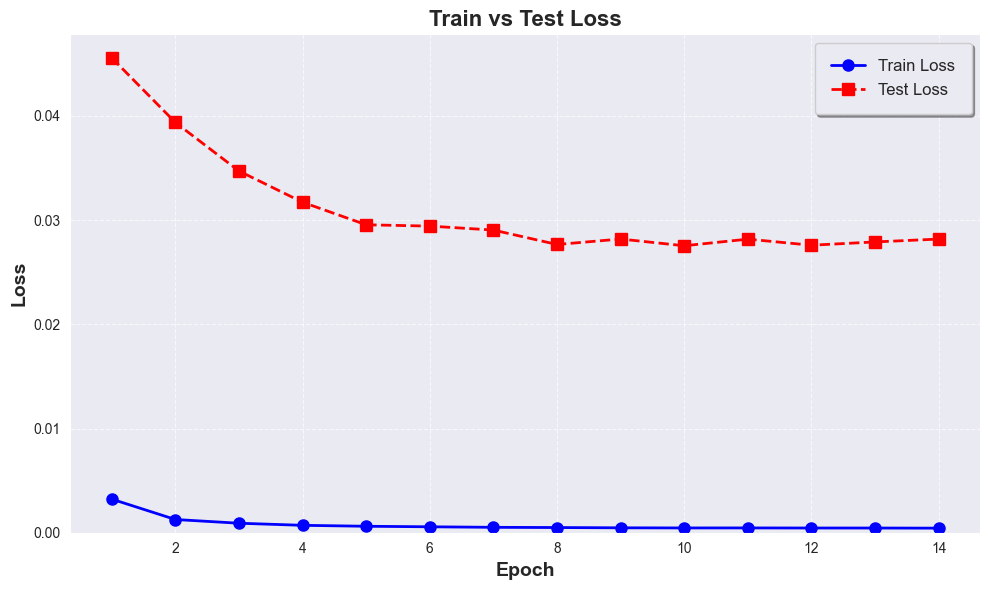
\includegraphics[width=1\textwidth]{train_vs_test.png}
    \caption{Évolution des fonctions de perte (train et test) sur la configuration de base}
    \label{fig:train_vs_test}
\end{figure}

On peut observer sur la figure \ref{fig:train_vs_test} que les deux courbes évoluent de façon décroissante et convergent progressivement vers zéro. On remarque toutefois que cette décroissance ralentit considérablement à partir de la cinquième époque, où les variations deviennent très faibles, indiquant que le modèle atteint un plateau dans son apprentissage.

\newpage
\subsection{Setup inversé}

Pour cette deuxième configuration, nous avons appliqué les mêmes fonctions d'apprentissage, mais en inversant délibérément les données d'entraînement et de test, de sorte que le corpus de test soit plus volumineux que celui d'entraînement. Cette approche non conventionnelle vise à étudier l'impact de la taille des ensembles de données sur l'apprentissage.

\begin{figure}[H]
    \centering
    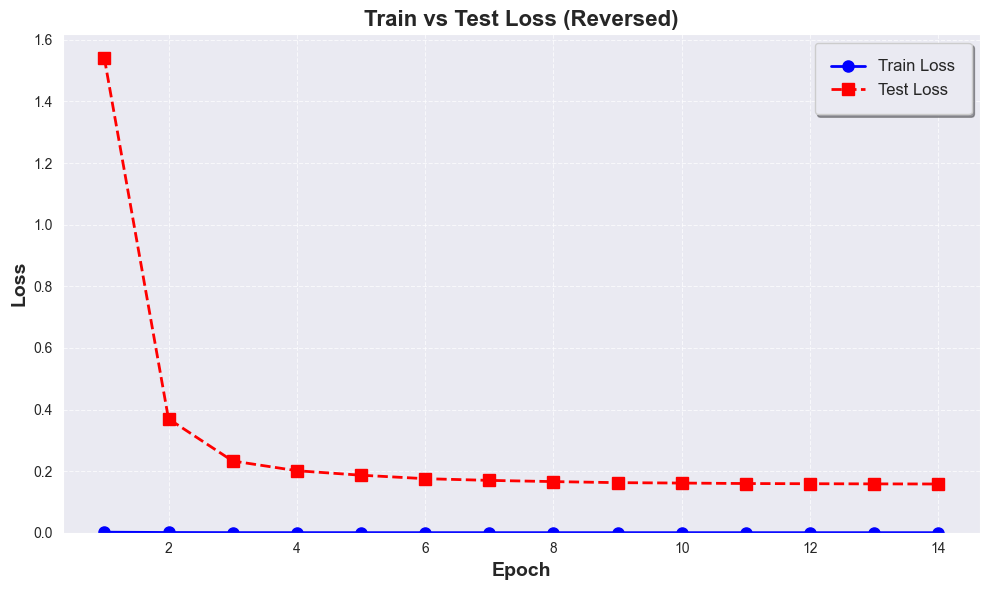
\includegraphics[width=1\textwidth]{train_vs_test_reversed.png}
    \caption{Évolution des fonctions de perte (train et test) sur la configuration inversée}
    \label{fig:train_vs_test_reversed}
\end{figure}

Ce second graphique (\ref{fig:train_vs_test_reversed}) révèle une évolution globalement similaire à celle de la configuration de base. Cependant, on observe une chute particulièrement brutale entre la première et la deuxième époque. Cette discontinuité s'explique par la valeur particulièrement élevée de la fonction de perte lors de la première époque, phénomène directement lié à la taille réduite du jeu de données utilisé pour l'entraînement, qui ne permet pas une initialisation optimale des poids du réseau.

\newpage
\subsection{Setup sans 'Dropout'}
\label{Setup_nd}

Dans le cadre de cette troisième configuration, nous avons délibérément désactivé les fonctions 'Dropout' de la classe \textit{Net} afin d'observer l'impact de cette technique de régularisation.\\
Le \textbf{Dropout} est une technique cruciale en apprentissage profond permettant de réduire le surapprentissage (overfitting) en désactivant temporairement et aléatoirement certains neurones et leurs connexions pendant la phase d'entraînement. Cette méthode force le réseau à développer des caractéristiques plus robustes et moins spécifiques aux données d'entraînement.

\begin{figure}[H]
    \centering
    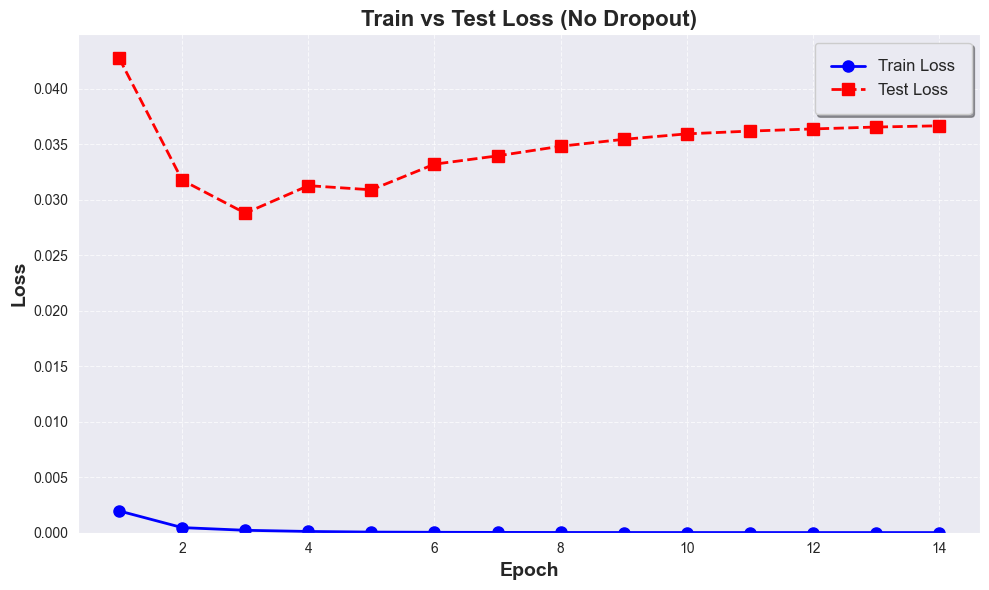
\includegraphics[width=1\textwidth]{train_vs_test_nd.png}
    \caption{Évolution des fonctions de perte (train et test) sans la régularisation par dropout}
    \label{fig:train_vs_test_nd}
\end{figure}

Cette fois-ci, le graphique \ref{fig:train_vs_test_nd} révèle une situation nettement différente et très instructive. Si la courbe d'entraînement (\textit{train}) continue de converger vers zéro comme attendu, on observe en revanche un comportement problématique sur la courbe de test. En effet, à partir de la troisième époque, la fonction de perte sur les données de test augmente continuellement, ce qui constitue un indicateur clair de surapprentissage (overfitting). Le réseau devient progressivement trop spécialisé sur les données d'entraînement et perd en capacité de généralisation sur de nouvelles données, démontrant ainsi l'importance cruciale du dropout comme mécanisme de régularisation.

\newpage
\subsection{Setup inversé et sans 'Dropout'}

Pour cette quatrième et dernière configuration, nous avons combiné les deux modifications précédentes : la désactivation du mécanisme de 'Dropout' et l'inversion des ensembles de données d'entraînement et de test. Cette configuration nous permet d'étudier l'interaction entre ces deux facteurs.

\begin{figure}[H]
    \centering
    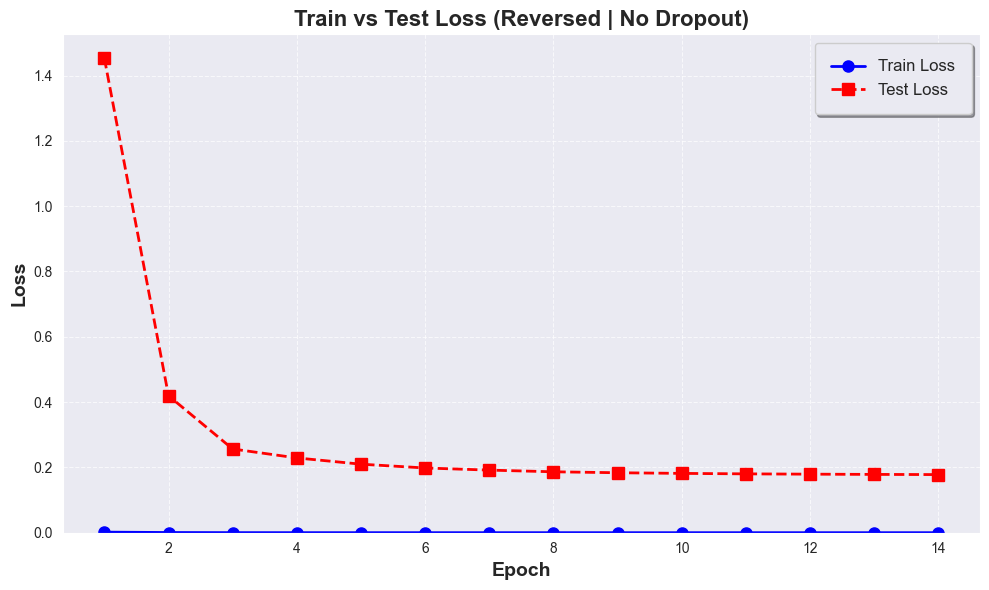
\includegraphics[width=1\textwidth]{train_vs_test_reversed_nd.png}
    \caption{Évolution des fonctions de perte (train et test) avec données inversées et sans régularisation par dropout}
    \label{fig:train_vs_test_reversed_nd}
\end{figure}

Le graphique \ref{fig:train_vs_test_reversed_nd} présente des caractéristiques relativement similaires à celles du graphique \ref{fig:train_vs_test_reversed}, avec notamment une fonction de perte particulièrement élevée lors de la première époque pour les données de test.

\newpage
\subsection{Conclusion}

Afin de tirer des conclusions significatives, nous allons maintenant procéder à une analyse comparative approfondie des différentes configurations expérimentales.

\begin{figure}[H]
    \centering
    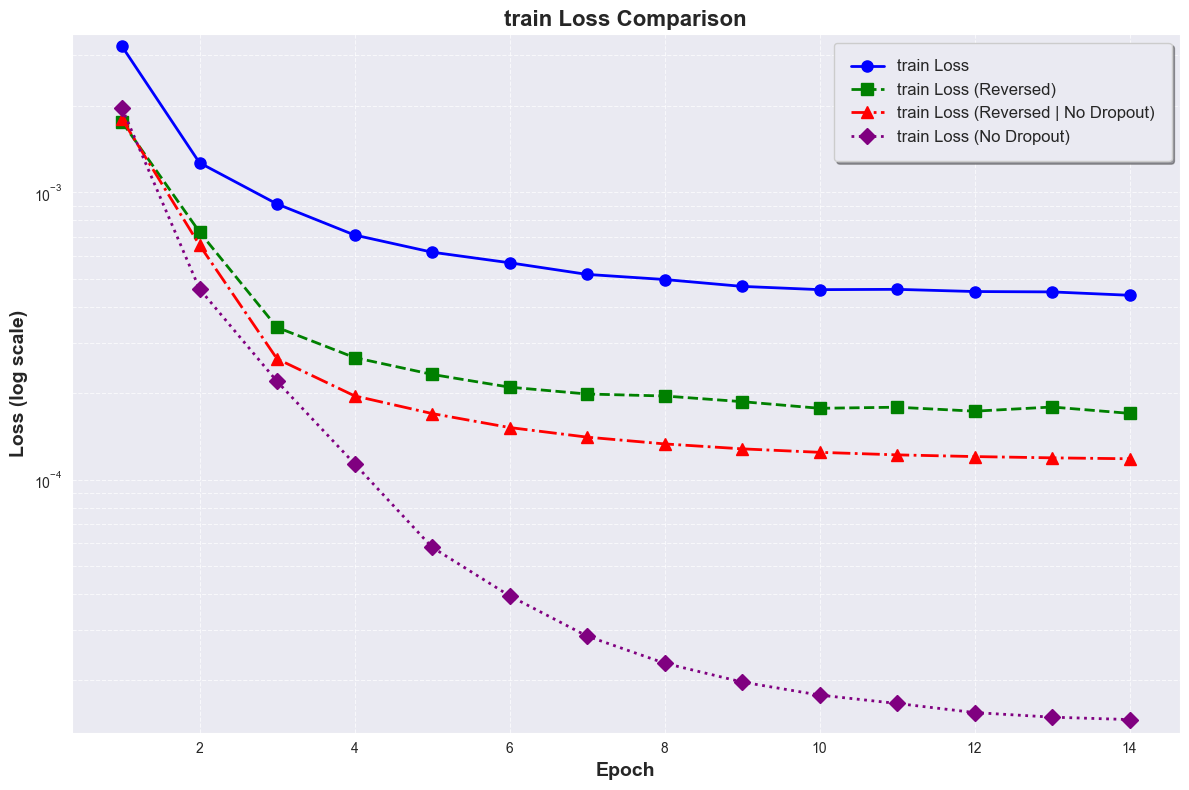
\includegraphics[width=1\textwidth]{train_compare.png}
    \caption{Analyse comparative de l'évolution des fonctions de perte d'entraînement}
    \label{fig:train_compare}
\end{figure}

L'analyse des quatre courbes d'entraînement révèle que toutes les configurations présentent une tendance décroissante de la fonction de perte, ce qui est cohérent avec un processus d'apprentissage fonctionnel. On remarque toutefois que les configurations sans dropout atteignent des valeurs de perte sensiblement plus faibles que les configurations avec dropout. Cette observation est particulièrement intéressante car elle illustre parfaitement le compromis fondamental entre la performance sur les données d'entraînement et la capacité de généralisation du modèle.

\begin{figure}[H]
    \centering
    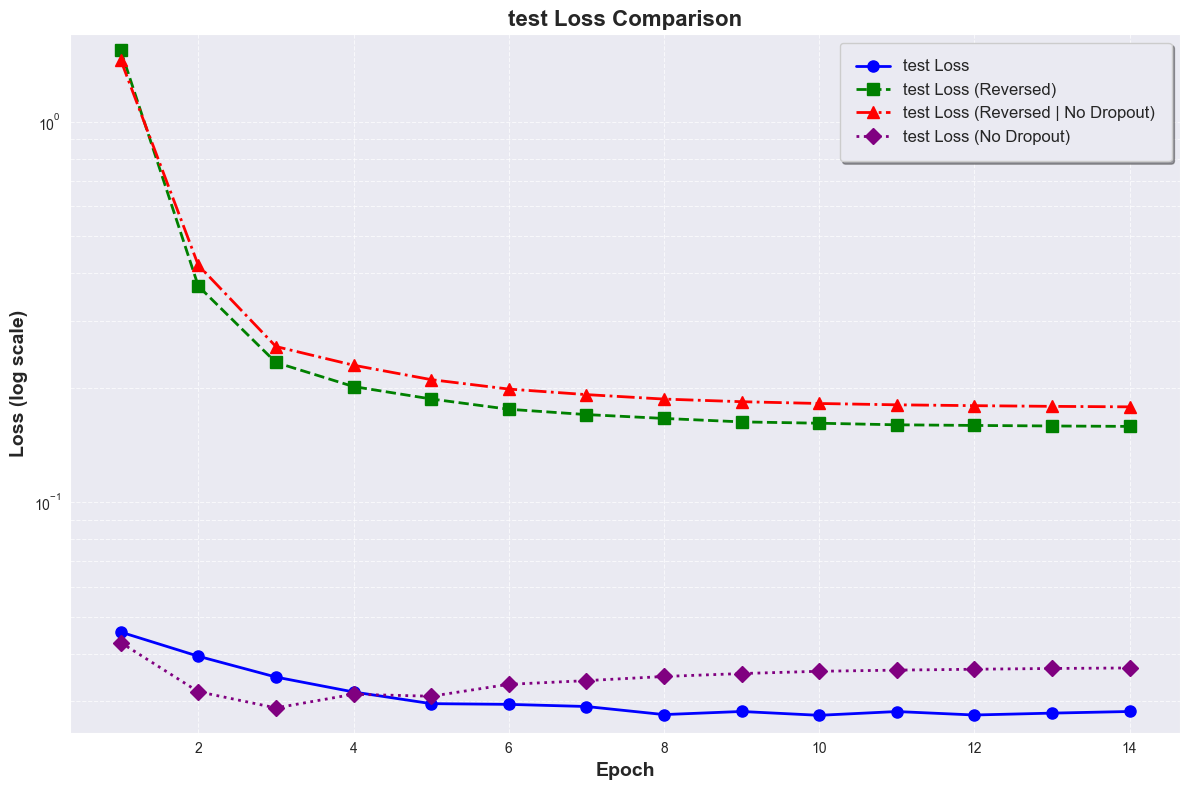
\includegraphics[width=1\textwidth]{test_compare.png}
    \caption{Analyse comparative de l'évolution des fonctions de perte de test}
    \label{fig:test_compare}
\end{figure}

Pour la phase de test, nous observons des résultats très différents. Les configurations avec données inversées montrent des pertes plus élevées que les configurations standards, soulignant l'importance d'avoir un ensemble d'entraînement suffisamment grand. De plus, on remarque que la configuration sans dropout montre une courbe qui remonte, contrairement aux configurations avec dropout qui continuent de descendre vers zéro. Ceci démontre clairement que le dropout joue un rôle essentiel pour éviter le surapprentissage et améliorer la capacité du modèle à généraliser sur de nouvelles données.

En conclusion, cette étude comparative nous permet de dégager plusieurs enseignements fondamentaux :

\begin{itemize}
    \item Lorsque le réseau apprend efficacement, la fonction de perte sur les données d'entraînement diminue progressivement et tend asymptotiquement vers zéro, indiquant une amélioration continue de la capacité prédictive du modèle sur les exemples connus.
    \item La fonction de perte sur les données de test suit généralement une trajectoire similaire dans un apprentissage optimal, mais peut présenter une augmentation significative en cas de surapprentissage (comme clairement démontré dans la configuration \ref{Setup_nd}), signalant une détérioration de la capacité de généralisation du modèle.
    \item L'inversion des ensembles de données d'entraînement et de test s'avère être une stratégie sous-optimale, générant systématiquement des fonctions de perte plus élevées pour la phase de test, ce qui souligne l'importance cruciale d'un ensemble d'entraînement suffisamment riche et représentatif.
    \item Le mécanisme de dropout démontre son efficacité en tant que technique de régularisation, permettant de maintenir une bonne capacité de généralisation au prix d'une légère diminution des performances sur les données d'entraînement, illustrant parfaitement le compromis biais-variance en apprentissage automatique.
\end{itemize}

\section{Perception acoustique et multimodale}

Cette partie traite de la perception acoustique et de la reconnaissance multimodale. Nous explorons les concepts fondamentaux de l'analyse et de la reconnaissance de signaux audio, en utilisant le jeu de données AudioMNIST, qui contient des enregistrements de chiffres de 0 à 9 prononcés par différents locuteurs. Nous abordons la visualisation et le prétraitement des signaux audio, l'analyse des spectrogrammes et la construction d'un modèle de reconnaissance des chiffres prononcés. Enfin, nous proposons une approche multimodale combinant reconnaissance visuelle (MNIST) et auditive (AudioMNIST).

\subsection{Exploration du jeu de données AudioMNIST}
\label{subsec:exploration}

Le jeu de données AudioMNIST contient des enregistrements audio de chiffres prononcés. Dans notre configuration, nous utilisons un sous-ensemble de 3000 fichiers.

\subsubsection{Structure des fichiers audio}
\label{subsubsec:structure}

Le nom de chaque fichier audio suit le format: \texttt{[chiffre]\_[locuteur]\_[répétition].wav}, où:
\begin{itemize}
    \item \texttt{[chiffre]} représente le chiffre prononcé (0-9)
    \item \texttt{[locuteur]} est l'identifiant du locuteur
    \item \texttt{[répétition]} est le numéro de répétition (0-50)
\end{itemize}
\newpage
\subsection{Visualisation des signaux audio}
\label{sec:visualisation}

Plusieurs méthodes de visualisation ont été explorées pour analyser les signaux audio.
Elles permettent de mieux comprendre les caractéristiques des signaux audio:
\begin{itemize}
    \item Représentation temporelle de la forme d'onde
    \item Spectrogramme Mel avec échelle en décibels
    \item Affichage des informations techniques (taux d'échantillonnage, durée, etc.)
\end{itemize}

\begin{figure}[H]
    \centering
    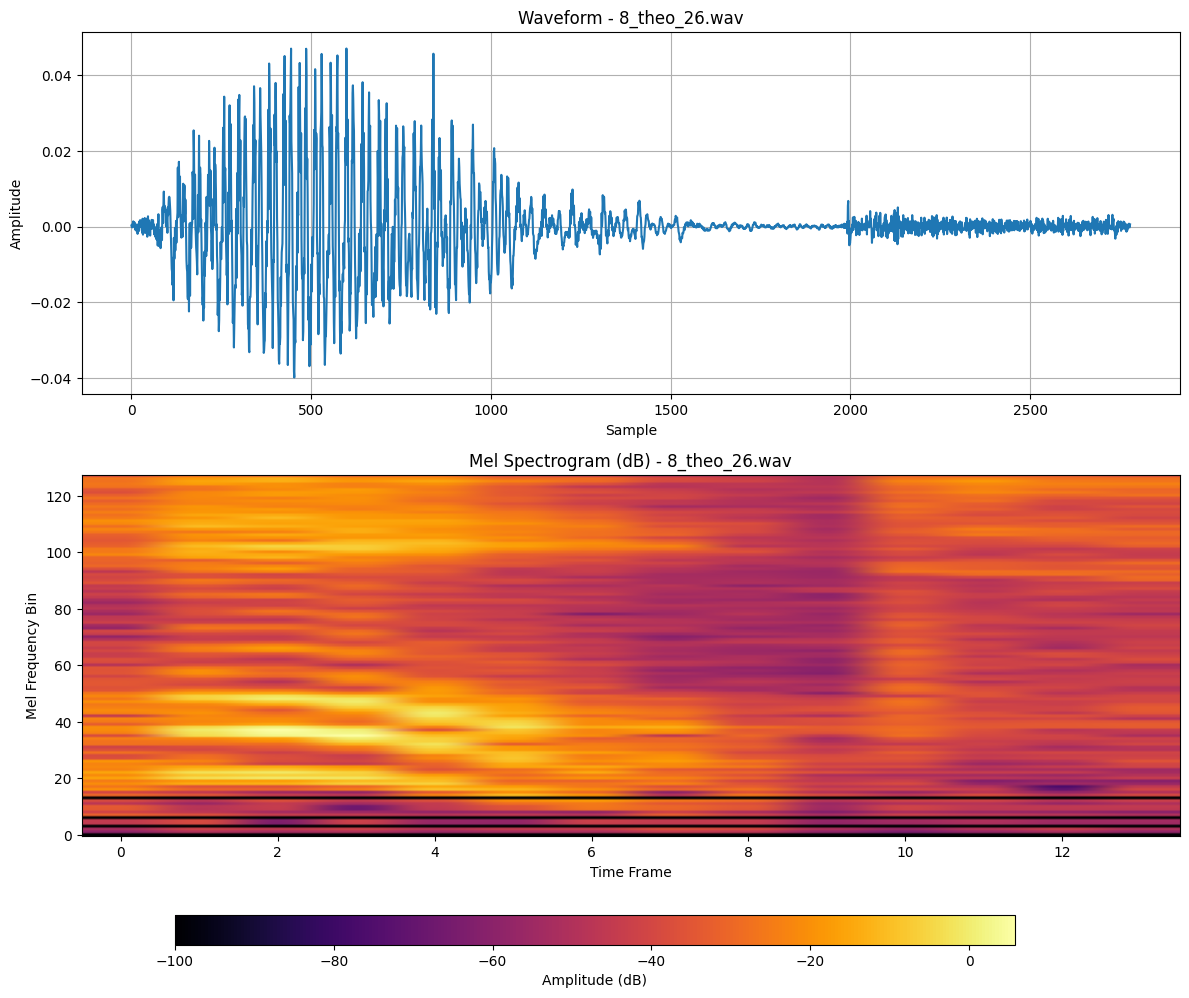
\includegraphics[width=1\textwidth]{WaveSpectro_1.png}
    \caption{Visualisation combinée: forme d'onde (haut) et spectrogramme Mel (bas) d'un fichier audio "8\_theo\_26.wav"}
    \label{fig:waveform_spec_1}
\end{figure}

Pour chaque fichier analysé, les informations suivantes ont été extraites:
\begin{itemize}
    \item Taux d'échantillonnage: 8000 Hz
    \item Forme de l'onde: 1 canal audio, durée variable (~2500-2800 échantillons)
    \item Forme du spectrogramme: 128 bandes de fréquences, ~13-14 fenêtres temporelles
    \item Durée moyenne: ~0.3-0.35 secondes
\end{itemize}

\begin{table}[H]
    \centering
    \begin{tabular}{|l|c|}
        \hline
        \textbf{Paramètre} & \textbf{Valeur} \\
        \hline
        Fichier & \texttt{8\_theo\_26.wav} \\
        Taux d’échantillonnage & 8000 Hz \\
        Forme de l’onde & [1, 2779] \\
        Forme du spectrogramme & [1, 128, 14] \\
        Durée de l’audio & 0.35 s \\
        \hline
    \end{tabular}
    \caption{Caractéristiques du 1er fichier audio analysé.}
    \label{tab:audio_info}
\end{table}

La visualisation des signaux audio permet de mieux comprendre leurs caractéristiques et d’analyser leur contenu spectral. Deux méthodes sont utilisées :

\begin{itemize}
    \item \textbf{Représentation temporelle} : affichage de la forme d’onde.
    \item \textbf{Spectrogramme Mel} : représentation spectrale avec échelle en décibels.
\end{itemize}

\subsubsection{Forme d’onde}

La Figure~\ref{fig:waveform_spec_1} présente une visualisation combinée de la forme d’onde et du spectrogramme Mel pour le fichier audio \texttt{8\_theo\_26.wav}.

\begin{itemize}
    \item \textbf{Axe des abscisses (X)} : Indice des échantillons audio.
    \item \textbf{Axe des ordonnées (Y)} : Amplitude du signal audio.
    \item \textbf{Interprétation} : Cette représentation permet d'observer l'intensité du signal au fil du temps. Cependant, elle ne donne aucune information sur la répartition des fréquences contenues dans le son. Par exemple, deux sons ayant des fréquences différentes mais des amplitudes similaires peuvent avoir des formes d’onde visuellement proches.
\end{itemize}

\subsubsection{Spectrogramme Mel}
\begin{itemize}
    \item \textbf{Axe des abscisses (X)} : Temps divisé en fenêtres successives.
    \item \textbf{Axe des ordonnées (Y)} : Bandes de fréquences sur l’échelle Mel.
    \item \textbf{Interprétation des couleurs}
    Les couleurs du spectrogramme indiquent l'intensité du signal dans différentes bandes de fréquences :
    \begin{itemize}
        \item \textbf{Zones jaunes / blanches} : Correspondent aux fréquences avec une intensité élevée. Elles indiquent les composantes dominantes du son.
        \item \textbf{Zones violettes / noires} : Correspondent aux fréquences avec une intensité faible. Elles représentent les zones silencieuses ou les parties du spectre où l’énergie est très faible.
    \end{itemize}
    \item \textbf{Interprétation} : Contrairement à la forme d’onde, le spectrogramme Mel montre la distribution des fréquences au fil du temps, ce qui est essentiel pour l’analyse acoustique.
\end{itemize}

\subsubsection{Conclusion}

La combinaison de ces deux représentations permet une analyse complète du signal audio. La forme d’onde fournit des informations globales sur l’intensité du signal, tandis que le spectrogramme Mel met en évidence les variations fréquentielles au fil du temps.

\subsection{Préparation des données d'entraînement et de test}
\label{sec:preparation}

\subsubsection{Séparation train/test}
\label{subsec:split}

Le script \texttt{SplitTrainTest\_original.py} a été utilisé pour diviser le jeu de données en deux sous-ensembles : 75\% des données pour l'entraînement et 25\% pour les tests, contrairement à la répartition 80/20 vue précédemment. Cette séparation est réalisée de manière aléatoire tout en garantissant une répartition équilibrée des classes. 

Pour cela, l'ensemble des données est préalablement mélangé afin d'assurer une représentation relativement équitable de chaque modalité cible dans les ensembles d'entraînement et de test.

\subsubsection{Analyse de la répartition des données}
\label{subsec:analyse_repartition}

L'analyse des fichiers CSV générés confirme que:
\begin{itemize}
    \item Ensemble d'entraînement: 2250 échantillons (75\%)
    \item Ensemble de test: 750 échantillons (25\%)
    \item Les deux ensembles contiennent des enregistrements de 6 locuteurs différents
    \item La répartition des chiffres est parfaitement équilibrée dans le jeu complet, et relativement équilibrée dans les sous-ensembles de données générées aléatoirement. 
\end{itemize}

\begin{table}[H]
    \centering
    \label{tab:data_distribution}
    \begin{minipage}{0.48\textwidth}
        \centering
        \caption{Test set (750 échantillons)}
        \begin{tabular}{|c|c|c|}
            \hline
            label & Count & Proportion \\
            \hline
            5 & 84 & 0.112 \\
            0 & 81 & 0.108 \\
            4 & 77 & 0.102 \\
            8 & 76 & 0.101 \\
            9 & 75 & 0.100 \\
            1 & 73 & 0.097 \\
            6 & 73 & 0.097 \\
            2 & 72 & 0.096 \\
            3 & 70 & 0.093 \\
            7 & 69 & 0.092 \\
            \hline
        \end{tabular}
    \end{minipage}\hfill
    \begin{minipage}{0.48\textwidth}
        \centering
        \caption{Train set (2250 échantillons)}
        \begin{tabular}{|c|c|c|}
            \hline
            label & Count & Proportion \\
            \hline
            7 & 231 & 0.102 \\
            3 & 230 & 0.102 \\
            2 & 228 & 0.101 \\
            1 & 227 & 0.100 \\
            6 & 227 & 0.100 \\
            9 & 225 & 0.100 \\
            8 & 224 & 0.099 \\
            4 & 223 & 0.099 \\
            0 & 219 & 0.097 \\
            5 & 216 & 0.096 \\
            \hline
        \end{tabular}
    \end{minipage}
\end{table}

\subsection{Etude du modèle}
\label{subsec:etude_model}

\subsubsection{Block 11}
Le block 11 définit une classe CNN (Convolutional Neural Network), contenant une initialisation et une méthode :
\begin{itemize}
    \item L'initialisation définit une séquence d'opérations comme l'algorithme ConvNet, utilisant des méthodes héritées de \texttt{nn.Module}. Elle définit l'architecture du réseau de neurones, ses couches :
    \begin{enumerate}
        \item Convolution 2D, avec 1 canal d'entrée, 10 de sortie et un noyau de taille $7 \times 7$ et un pas de 3. Cette couche produit 10 feature maps pour chaque donnée d'entrée, le filtre faisant cela est de taille $7 \times 7$ permettant de détecter des patterns dans les données.
        \item Fonction d'activation ReLU, appliquée à la 1\iere{} couche (introduit de la non-linéarité).
        \item Convolution 2D, avec 10 canaux d'entrée, 10 de sortie et un noyau de taille $5 \times 5$ et un pas de 2. La couche prend en entrée les 10 features maps de la couche précédente, le filtre appliqué aux feature maps est de taille $5 \times 5$, appliqué à chaque feature map il effectue des convolutions sur les données. Le pas et le kernel diminués permettent de diminuer la taille de la sortie de la 2\ieme{} couche comparée à la 1\iere{}.
        \item Fonction d'activation ReLU, appliquée à la 2\ieme{} couche.
        \item Aplatissement des données (couche de neurones) en un vecteur 1D.
        \item Application d'une fonction affine linéaire aux données, prend en entrée un vecteur de grande taille ($38 \times 19 \times 10$), et donne un vecteur de taille 10 en sortie.
    \end{enumerate}
    \item La méthode \texttt{forward} permet de passer des données dans le réseau défini précédemment. On passe une donnée X dans le réseau et on sort les logits, score brut (avant l'application de la fonction d'activation) pour chaque classe prédite.
\end{itemize}

\subsubsection{Block 12}
Le block 12 crée un modèle à partir de la classe CNN. Ce modèle est transféré sur un dispositif qui sera le GPU s'il y en a un, et le CPU sinon.

\subsubsection{Block 13}
Le block 13 initialise la fonction de perte d'entropie croisée de PyTorch. Elle permet de mesurer les écarts entre prédictions du modèle et vraies étiquettes des données, la Loss. Cela permet d'évaluer la performance du modèle créé. Plus la Loss est faible, plus le modèle est bon.

Ensuite, le block contient un optimiseur de modèle via un gradient. Il permet d'ajuster les poids du modèle pour minimiser la Loss. Les paramètres du gradient sont : un taux d'apprentissage à 0.001 (taille des mises à jour de poids), et un momentum de 0.9 (aide à converger plus rapidement).
\newpage
\subsubsection{Block 14}
Ce block définit 2 fonctions :
\begin{itemize}
    \item La fonction \texttt{train}, utilise le modèle CNN prédéfini, l'optimiseur, la fonction permettant de calculer la Loss, et des données d'entrée.
    La fonction, pour des lots de données :
    \begin{enumerate}
        \item Charge les données (dans le format adapté au device (GPU ou CPU)) et les normalise,
        \item Utilise le modèle CNN en mode entraînement pour activer le calcul des gradients,
        \item Ensuite les opérations "Forward Pass" ont lieu : récupère les prédictions de labels faites par le modèle, calcule la loss,
        \item Met à jour les indicateurs globaux de la loss totale et du nombre de prédictions correctes,
        \item Enfin a lieu le "Backward Pass", on utilise la backpropagation via l'optimiseur gradient (reset du gradient, calculs des pertes pour les paramètres, mise à jour des paramètres du gradient),
        \item La fonction renvoie la perte moyenne et le score du modèle (précision).
    \end{enumerate}
    
    \item La fonction \texttt{test}, utilise le modèle CNN et la fonction de calcul de la Loss.
    La fonction, par lots :
    \begin{enumerate}
        \item Charge les données (dans le format adapté au device (GPU ou CPU)) et les normalise,
        \item Utilise le modèle CNN en mode évaluation sans activer le calcul des gradients,
        \item Ensuite on fait uniquement une opération "Forward Pass", on utilise le modèle et récupère les prédictions,
        \item Calcule la Loss de ce modèle et met à jour les indicateurs globaux,
        \item Enfin, la fonction renvoie la perte moyenne et le score du modèle (précision).
    \end{enumerate}
\end{itemize}

\subsubsection{Block 15}
Dans ce block, on utilise tous les éléments et fonctions définis précédemment. Pour 30 epochs, on entraîne et teste le modèle, en ajoutant tous les indicateurs de performance (loss et score de précision) à des listes pour les conserver.

\subsubsection{Architecture du modèle CNN}
\label{subsubsec:architecture}

Le modèle utilisé est un réseau de neurones convolutif (CNN) avec l'architecture suivante:

\begin{enumerate}
    \item \textbf{Première couche convolutive:}
    \begin{itemize}
        \item 1 canal d'entrée, 10 canaux de sortie
        \item Noyau de taille $7 \times 7$, et un pas de 3
        \item Détecte les motifs de base dans les spectrogrammes
    \end{itemize}
    
    \item \textbf{Fonction d'activation ReLU} après la première couche
    
    \item \textbf{Seconde couche convolutive:}
    \begin{itemize}
        \item 10 canaux d'entrée, 10 canaux de sortie
        \item Noyau de taille $5 \times 5$, pas de 2
        \item Traite les feature maps de la première couche
    \end{itemize}
    
    \item \textbf{Fonction d'activation ReLU} après la seconde couche
    
    \item \textbf{Aplatissement} des données en vecteur 1D
    
    \item \textbf{Couche fully connected} qui réduit le vecteur aplati à 10 sorties, une pour chaque chiffre
\end{enumerate}

\begin{figure}[H]
    \centering
    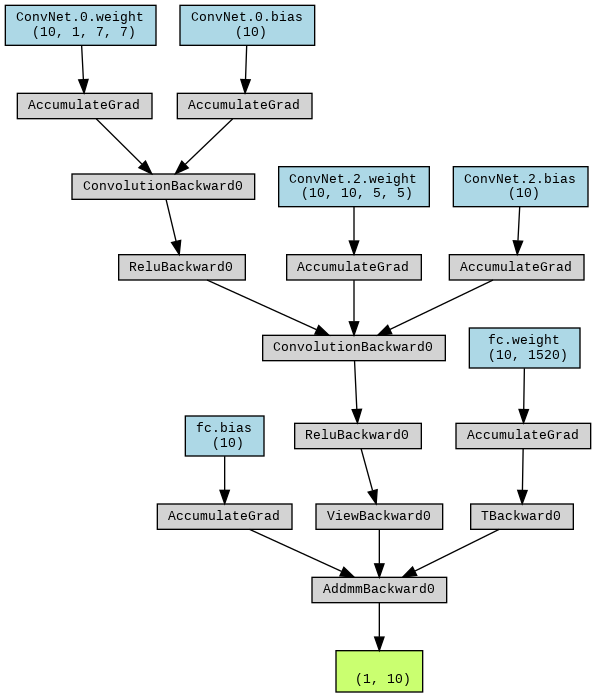
\includegraphics[width=0.9\textwidth]{Schema_CNN_Audio.png}
    \caption{Architecture du réseau de neurones convolutif utilisé pour la reconnaissance des chiffres prononcés}
    \label{fig:cnn_archi}
\end{figure}

\subsubsection{Quel est ce modèle ?}
\label{subsubsec:quel_modele}

Les blocs 11 à 15 décrivent un modèle de réseau de neurones convolutif (CNN) pour la classification multimodale d'images et de spectrogrammes audio. Le modèle est entraîné à l'aide de PyTorch, avec des fonctions de perte et des optimisateurs pour ajuster les poids du réseau. Le processus d'entraînement et de test est itératif, avec des évaluations de la performance à chaque époque pour suivre la précision et la perte du modèle.

\subsubsection{Fonction de perte et optimisation}
\label{subsubsec:loss_optim}

Le modèle utilise:
\begin{itemize}
    \item \textbf{Fonction de perte:} Cross-Entropy Loss, adaptée pour les problèmes de classification
    \item \textbf{Optimiseur:} Stochastic Gradient Descent (SGD) avec:
    \begin{itemize}
        \item Taux d'apprentissage: 0.001
        \item Momentum: 0.9 pour accélérer la convergence
    \end{itemize}
\end{itemize}

\subsubsection{Processus d'entraînement et d'évaluation}
\label{subsec:training}

Le processus comprend deux fonctions principales:
\begin{itemize}
    \item \textbf{Fonction train:}
    \begin{itemize}
        \item Active le mode entraînement du modèle
        \item Normalise les données d'entrée
        \item Effectue une passe avant pour obtenir les prédictions
        \item Calcule la perte et met à jour les indicateurs
        \item Effectue une passe arrière (backpropagation) pour ajuster les poids
    \end{itemize}
    
    \item \textbf{Fonction test:}
    \begin{itemize}
        \item Active le mode évaluation du modèle (sans calcul de gradients)
        \item Normalise les données d'entrée
        \item Effectue uniquement une passe avant
        \item Calcule la perte et les métriques de performance
    \end{itemize}
\end{itemize}

L'entraînement se déroule sur 30 époques, avec un suivi de la perte et de la précision pour les ensembles d'entraînement et de test.
\newpage
\subsection{Analyse des performances}
\label{subsec:performances}

Les courbes d'apprentissage montrent :

\begin{figure}[H]
    \centering
    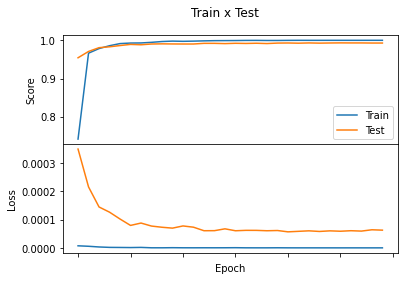
\includegraphics[width=0.8\textwidth]{learning_curves.png}
    \caption{Évolution de la précision et de la perte durant l'entraînement}
    \label{fig:curves}
\end{figure}

\begin{itemize}
    \item \textbf{Précision (accuracy) :}
    \begin{itemize}
        \item Ensemble d'entraînement : La précision atteint rapidement une valeur proche de 100\%, ce qui indique une excellente performance du modèle sur cet ensemble, un apprentissage quasi parfait sur l'ensemble d'entraînement..
        \item Ensemble de test : La précision se stabilise à une valeur élevée mais légèrement inférieure à celle de l'entraînement, ce qui reflète une généralisation correcte, bien que légèrement moins performante que sur l'ensemble d'entraînement.
    \end{itemize}
    
    \item \textbf{Perte (loss) :}
    \begin{itemize}
        \item Ensemble d'entraînement : La perte diminue rapidement et se stabilise à une valeur très basse, ce qui indique que le modèle s'adapte bien aux données d'entraînement.
        \item Ensemble de test : La perte continue de diminuer, mais elle reste plus élevée que celle observée pour l'entraînement, ce qui suggère un léger écart entre les performances sur les ensembles d'entraînement et de test. 
    \end{itemize}
    
    \item \textbf{Interprétation :} L'écart entre les performances d'entraînement et de test suggère un léger surapprentissage (overfitting). Cependant, étant donné que les résultats sur l'ensemble de test restent bons, cela montre que le modèle généralise correctement, bien que des ajustements pour limiter l'overfitting pourraient être nécessaires.
\end{itemize}


\subsection{Proposition d'un système multimodal}
\label{sec:multimodal}

L'objectif est de créer un système multimodal qui combine:
\begin{itemize}
    \item La reconnaissance visuelle des chiffres écrits (MNIST)
    \item La reconnaissance acoustique des chiffres prononcés (AudioMNIST)
\end{itemize}

Cette fusion vise à améliorer la performance globale du système en tirant parti de la complémentarité des deux modalités.

\subsubsection{Préparation des données}
\label{subsubsec:prep_multi}

\paragraph{MNIST (Images)}
\begin{itemize}
    \item Chargement via torchvision
    \item Normalisation des images
    \item Division en ensembles d'entraînement et de test
\end{itemize}

\paragraph{AudioMNIST (Audio)}
\begin{itemize}
    \item Uniformisation de la durée des signaux
    \item Conversion en MelSpectrogrammes
    \item Application d'une transformation logarithmique (pour plus de robustesse)
    \item Division en ensembles d'entraînement et de test
\end{itemize}

\paragraph{Extraction des Caractéristiques (features)}
\begin{itemize}
    \item Pour MNIST, les pixels des images constituent les features.
    \item Pour AudioMNIST, extraire des caractéristiques à partir des MelSpectrograms.
\end{itemize}

\subsubsection{Conception du modèle}
\label{subsubsec:conception}

\paragraph{Modèles indépendants}
\begin{itemize}
    \item \textbf{Modèle image:} CNN pour MNIST
    \item \textbf{Modèle audio:} CNN ou RNN pour AudioMNIST
\end{itemize}
\newpage
\paragraph{Stratégies de fusion}

\begin{figure}[H]
    \centering
    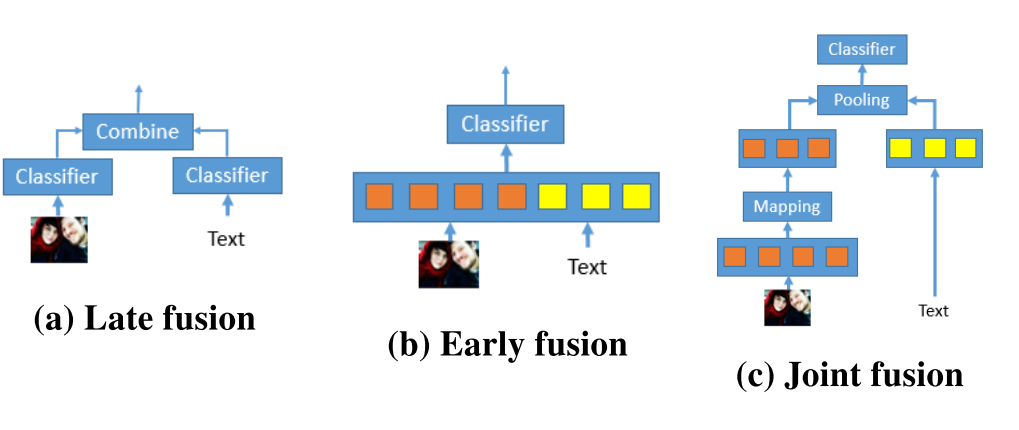
\includegraphics[width=0.9\textwidth]{fusion_strategies.png}
    \caption{Illustration des différentes stratégies de fusion multimodale}
    \label{fig:fusion}
\end{figure}

\begin{itemize}
    \item \textbf{Fusion précoce (Early fusion) (b):}
    \begin{itemize}
        \item Concaténation des caractéristiques brutes
        \item Permet d'apprendre des corrélations à bas niveau
        \item Nécessite d'harmoniser les dimensions des modalités
    \end{itemize}
    
    \item \textbf{Fusion intermédiaire (Joint fusion) (c):}
    \begin{itemize}
        \item Extraction séparée des caractéristiques pour chaque modalité
        \item Fusion des représentations obtenues
        \item Options : concaténation, couche d'attention
    \end{itemize}
    
    \item \textbf{Fusion tardive (Late fusion) (a):}
    \begin{itemize}
        \item Chaque modalité est traitée indépendamment par un classificateur
        \item Les prédictions finales sont combinées pour obtenir une décision finale
        \item Méthodes : moyenne pondérée, vote majoritaire
        \item Avantage : robuste en cas de défaillance d’une modalité
    \end{itemize}    
\end{itemize}

\paragraph{Architecture proposée}
\begin{itemize}
    \item Encodeurs spécifiques à chaque modalité  (CNN pour images, CNN/RNN pour audio)
    \item Mécanisme d'attention pour pondérer l'importance des modalités
    \item Couches fully connected finales pour la classification
\end{itemize}

\subsubsection{Entraînement et évaluation}
\label{subsubsec:train_eval}

\begin{itemize}
    \item Entraînement des modèles individuels
    \item Entraînement du modèle fusionné
    \item Comparaison des performances:
    \begin{itemize}
        \item Modèle visuel seul
        \item Modèle audio seul
        \item Modèle multimodal
    \end{itemize}
    \item Analyse des cas où une modalité est plus fiable que l'autre
\end{itemize}

\subsubsection{Optimisation}
\label{subsubsec:optimisation}

\begin{itemize}
    \item Expérimentation avec différentes architectures
    \item Ajustement des hyperparamètres
    \item Augmentation des données
    \item Raffinement de la stratégie de fusion
\end{itemize}

\begin{figure}[H]
    \centering
    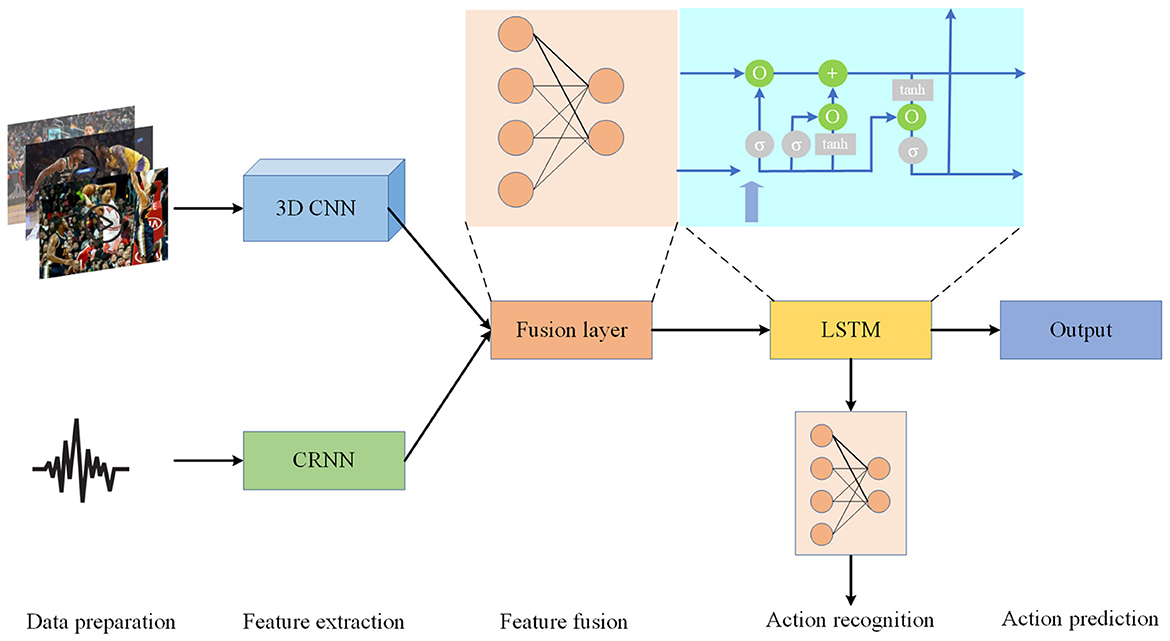
\includegraphics[width=0.9\textwidth]{multimodal_system.jpg}
    \caption{Architecture générale du système multimodal proposé}
    \label{fig:system}
\end{figure}

\newpage

\section{Analyse de la sensibilité des réseaux convolutifs}

Dans cette troisième et dernière partie, nous allons analyser la sensibilité des réseaux convolutifs à leur entrée sur une tâche de classification d’image de type ImageNet. L’objectif est de visualiser et de comprendre à quels pixels le réseau est sensible lors de la prise de décision de classification.

\subsection{Algorithmes de Class Activation Mapping (CAM)}

Les algorithmes de Class Activation Mapping (CAM) sont des techniques utilisées en vision par ordinateur pour visualiser les régions d'une image qui influencent le plus la décision d'un modèle de classification. Ces méthodes génèrent des cartes d'activation qui mettent en évidence les zones importantes de l'image pour une classe donnée.\\

Dans la page GitHub \href{https://github.com/utkuozbulak/pytorch-cnn-visualizations}{utkuozbulak/pytorch-cnn-visualizations}, différentes méthodes de Class Activation Mapping (CAM) sont présentées pour visualiser quelles régions d'une image influencent le plus la décision d'un modèle CNN :

\begin{itemize}
    \item \textbf{CAM} : Utilise une combinaison pondérée des activations de la dernière couche convolutionnelle pour générer une carte de chaleur des régions les plus influentes.
    \item \textbf{Grad-CAM} : Utilise les gradients de la classe cible par rapport aux cartes d'activation pour générer une carte de chaleur plus précise.
    \item \textbf{Grad-CAM++} : Améliore Grad-CAM en prenant en compte les contributions positives de chaque pixel avec des poids spécifiques.
    \item \textbf{Score-CAM} : Utilise les scores de prédiction pour évaluer l'importance des caractéristiques, évitant ainsi les coûts de calcul associés aux gradients.
\end{itemize}

\subsection{Activation d'une classe sur des images}

Nous allons maintenant nous intéresser à l'activation d'une classe sur différentes images. Notre étude utilisera trois images : 
\begin{itemize}
    \item Une image contenant un seul objet de la classe.
    \item Une image contenant plusieurs objets de la classe.
    \item Une image ne contenant aucun objet de la classe.
\end{itemize}

\subsubsection{Choix du setup}

Pour mener à bien cette étude, nous avons sélectionné un setup composé d'un modèle backbone, d'une méthode de CAM et d'une classe cible. Nos choix se sont portés sur : 
\begin{itemize}
    \item Le modèle \texttt{regnet\_y\_400mf}, qui offre un bon équilibre entre performance et efficacité.
    \item La méthode \textbf{Grad-CAM++}, car elle est l'une des méthodes les plus complètes tout en restant légère par rapport à Score-CAM.
    \item La classe à détecter sera \textit{tennis ball}.
\end{itemize}

\newpage

Voici les images utilisées pour l'étude :

\begin{table}[H]
    \centering
    \begin{tabular}{|c|c|c|}
      \hline
      \textbf{Un objet} & \textbf{Plusieurs objets} & \textbf{Aucun objet} \\
      \hline
      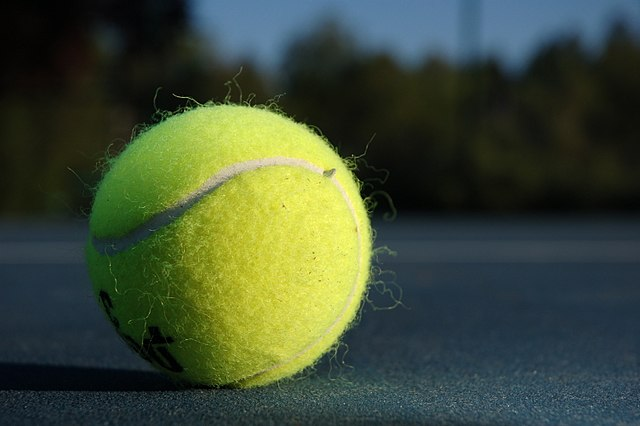
\includegraphics[width=0.3\textwidth]{tennis_ball.jpg} &
      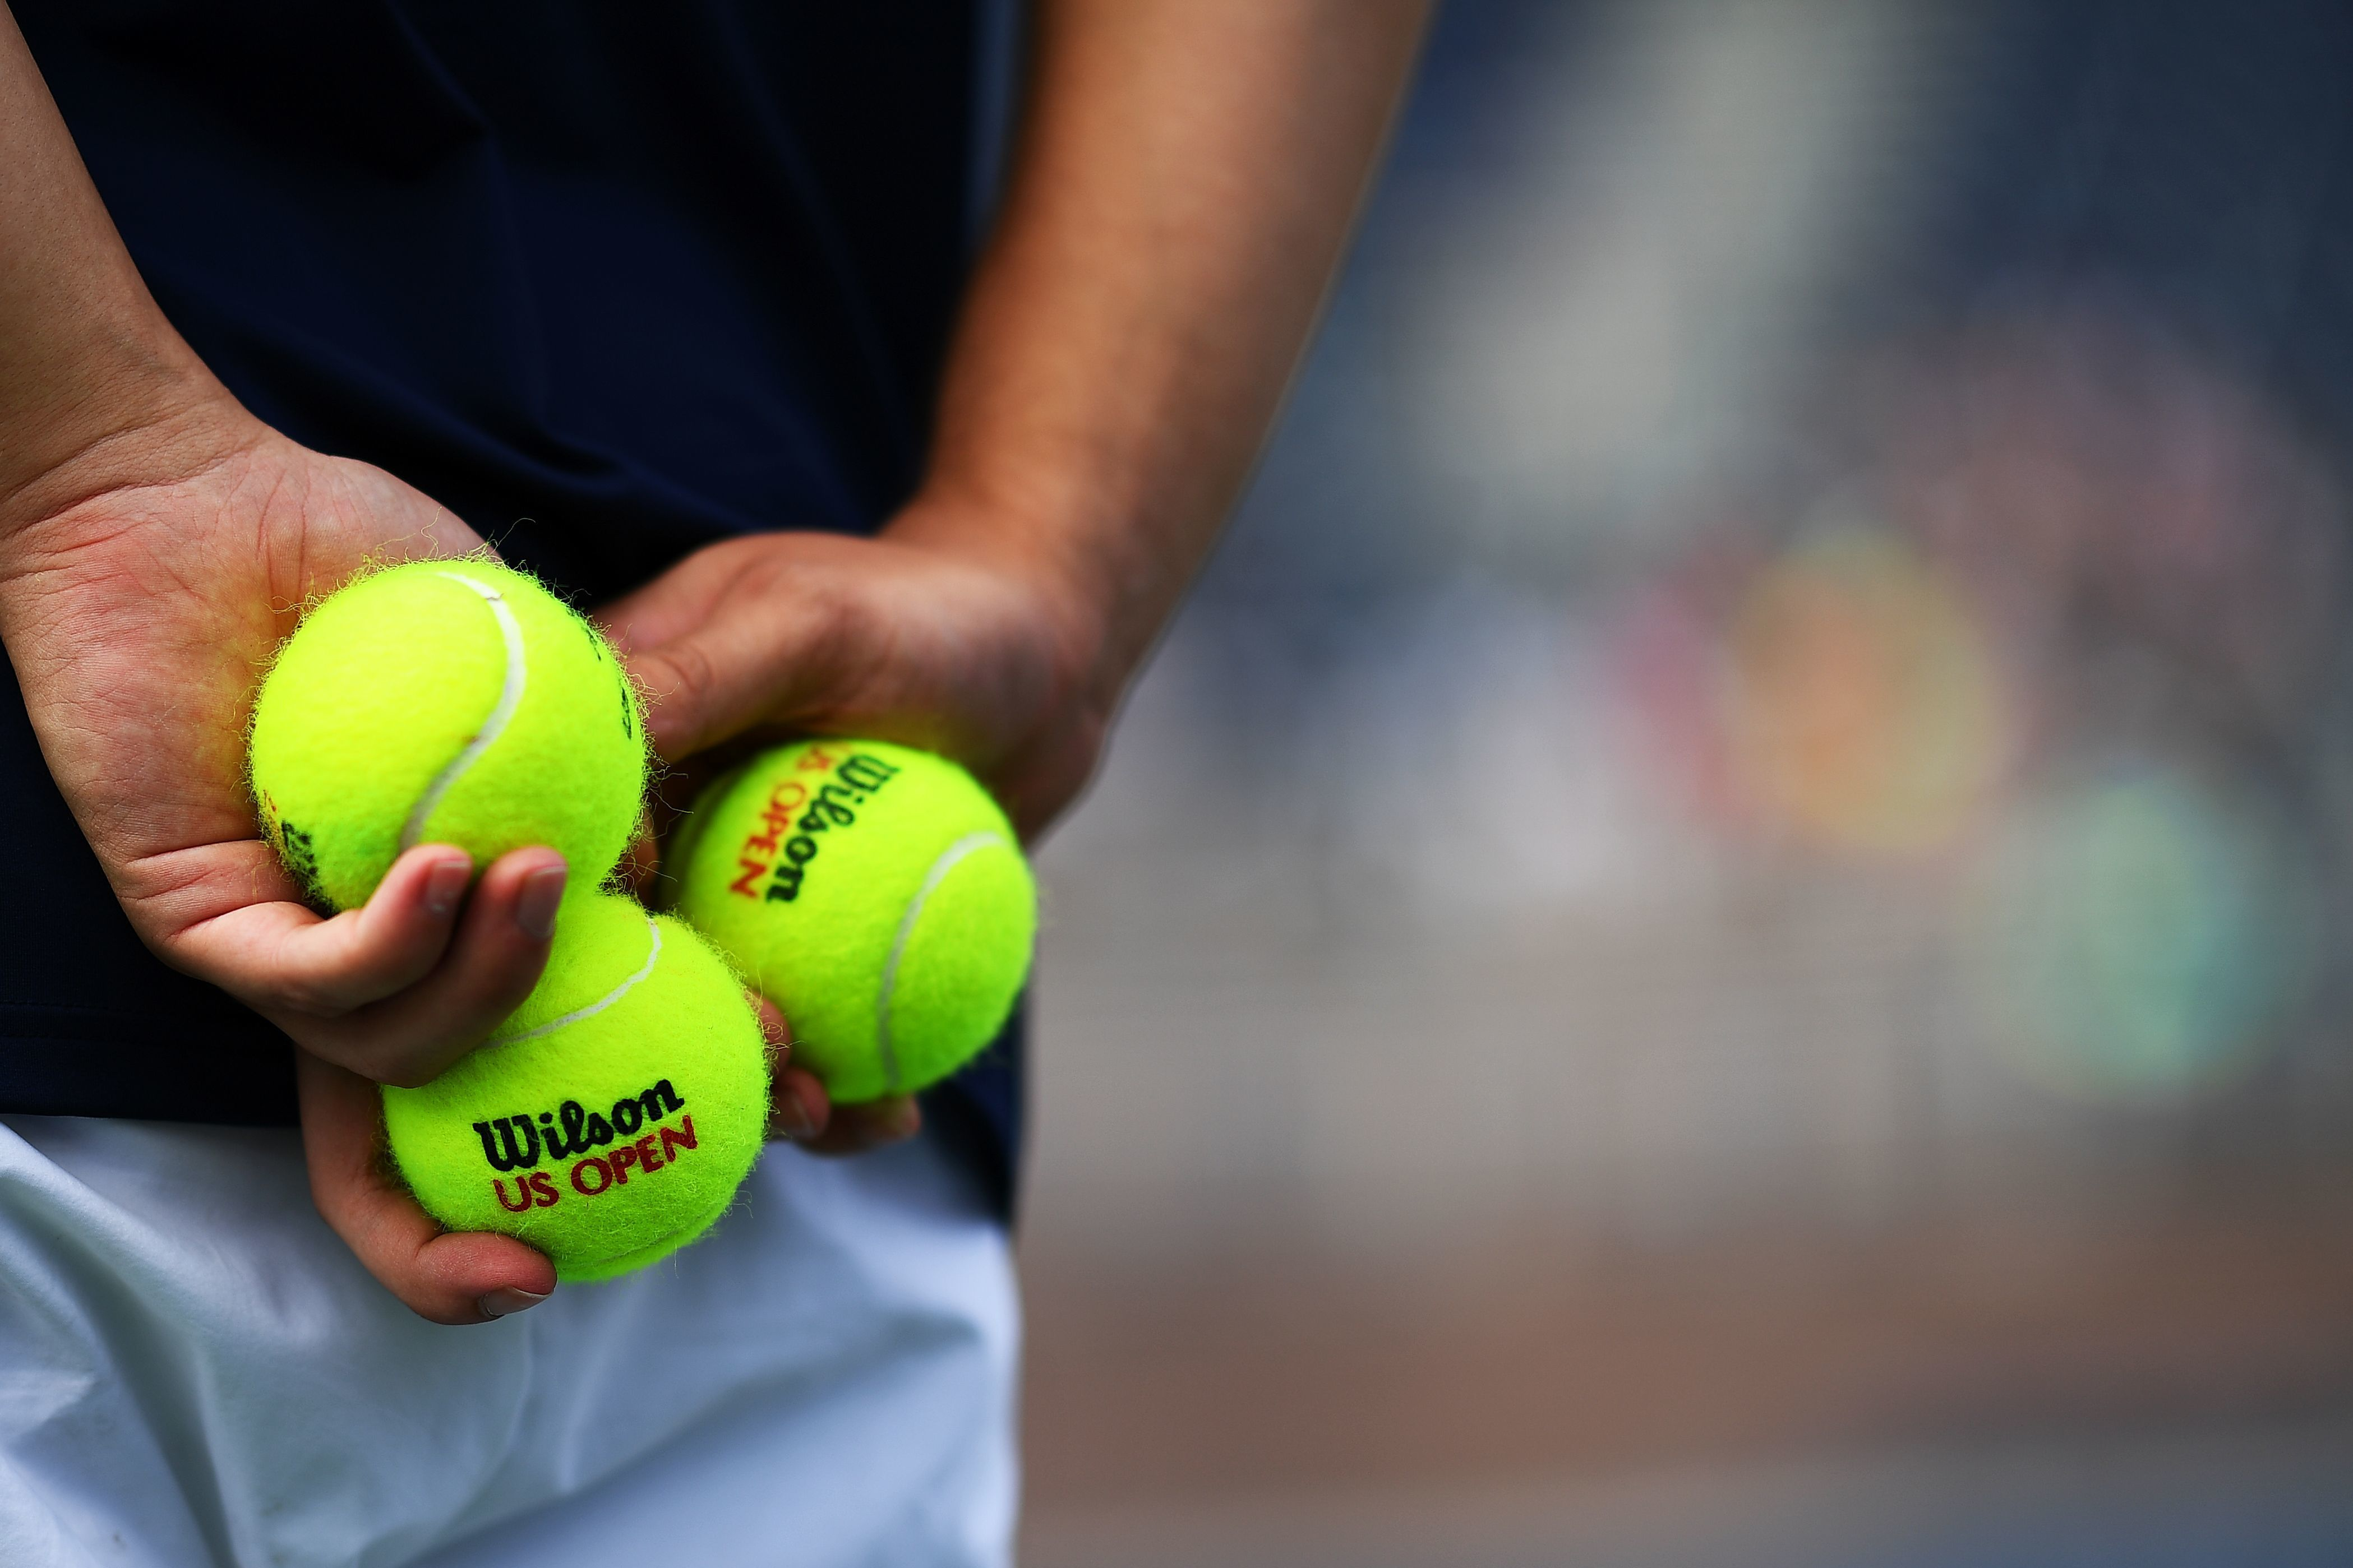
\includegraphics[width=0.3\textwidth]{tennis_balls.jpg} &
      \includegraphics[width=0.3\textwidth]{z.jpg} \\
      \hline
    \end{tabular}
    \caption{Images utilisées pour l'analyse CAM.}
    \label{tab:images_cam}
\end{table}

\subsubsection{Analyse des résultats}
\begin{figure}[H]
    \centering
    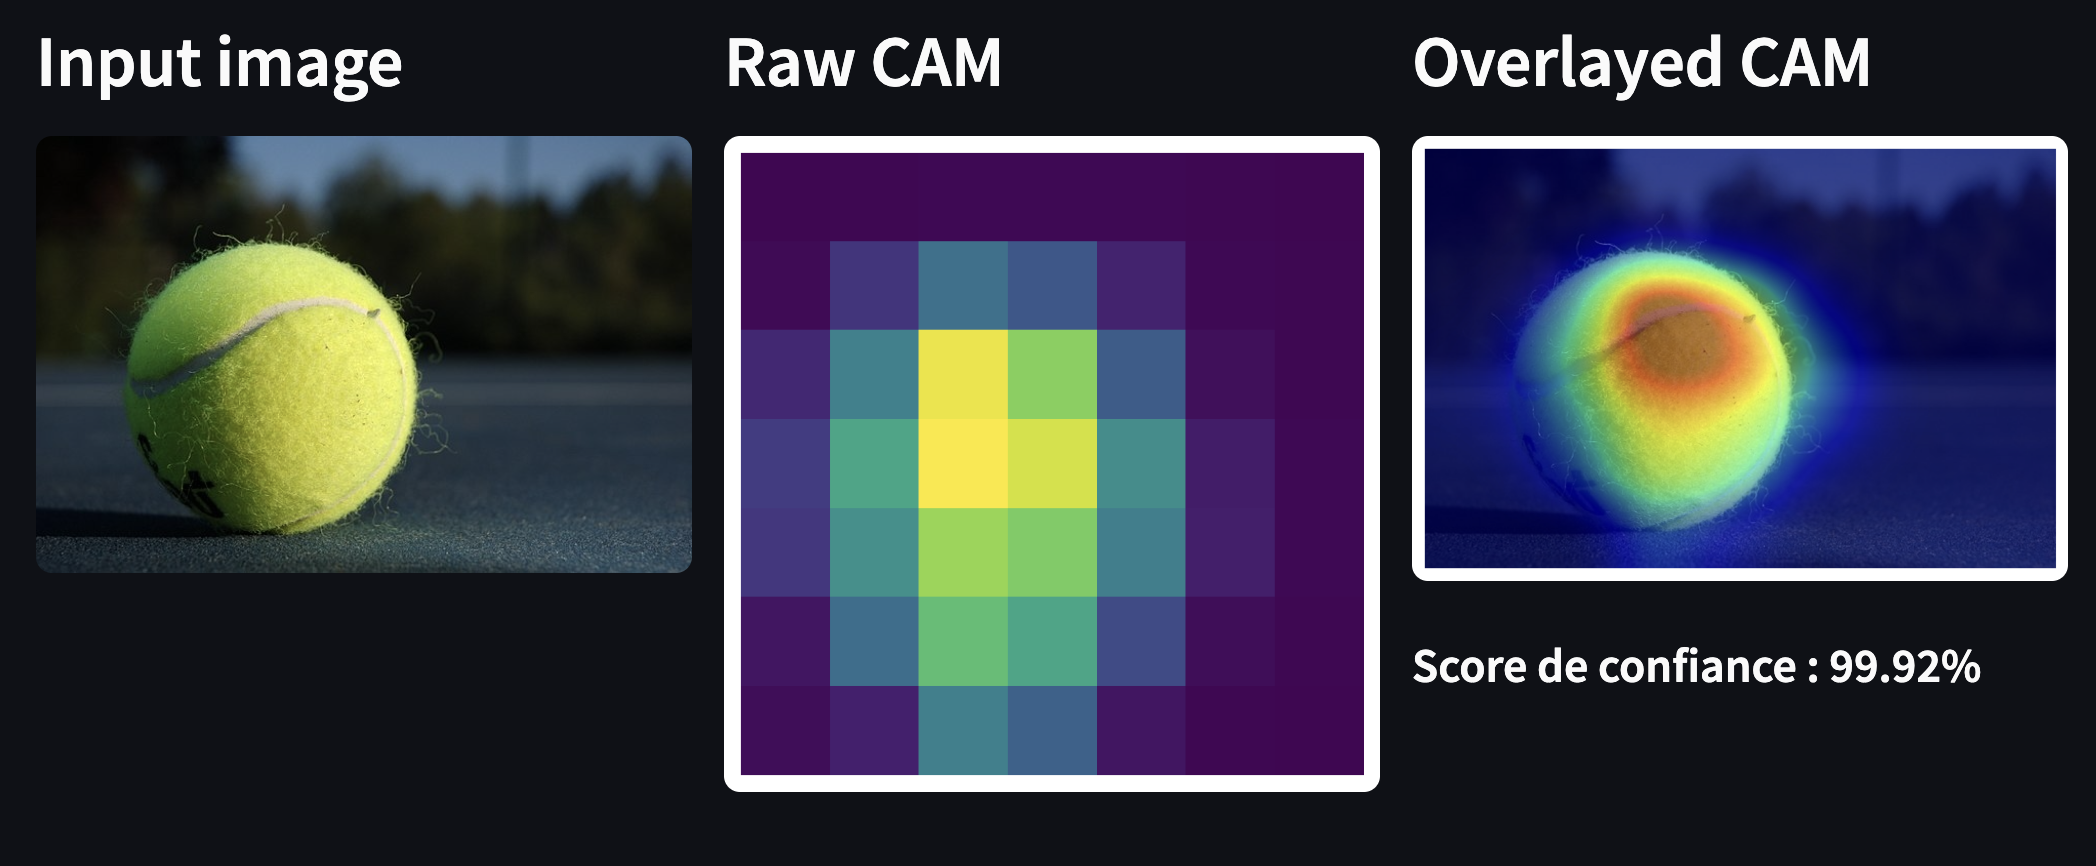
\includegraphics[width=0.9\linewidth]{CAM_tennis_ball.png}
    \caption{Résultat de l'activation pour une balle de tennis seule.}
\end{figure}
Pour la balle de tennis seule, le modèle identifie l'objet avec un score de confiance de \textbf{99.92\%}. La carte thermique dans la partie "Overlayed CAM" montre clairement les zones qui contribuent le plus à la classification, avec la région la plus brillante (jaune/rouge) concentrée précisément sur la balle de tennis. La carte d'activation brute ("Raw CAM") révèle les pixels activés avant lissage, indiquant que le modèle se concentre principalement sur la forme circulaire et la couleur jaune-vert caractéristique de la balle.

\begin{figure}[H]
    \centering
    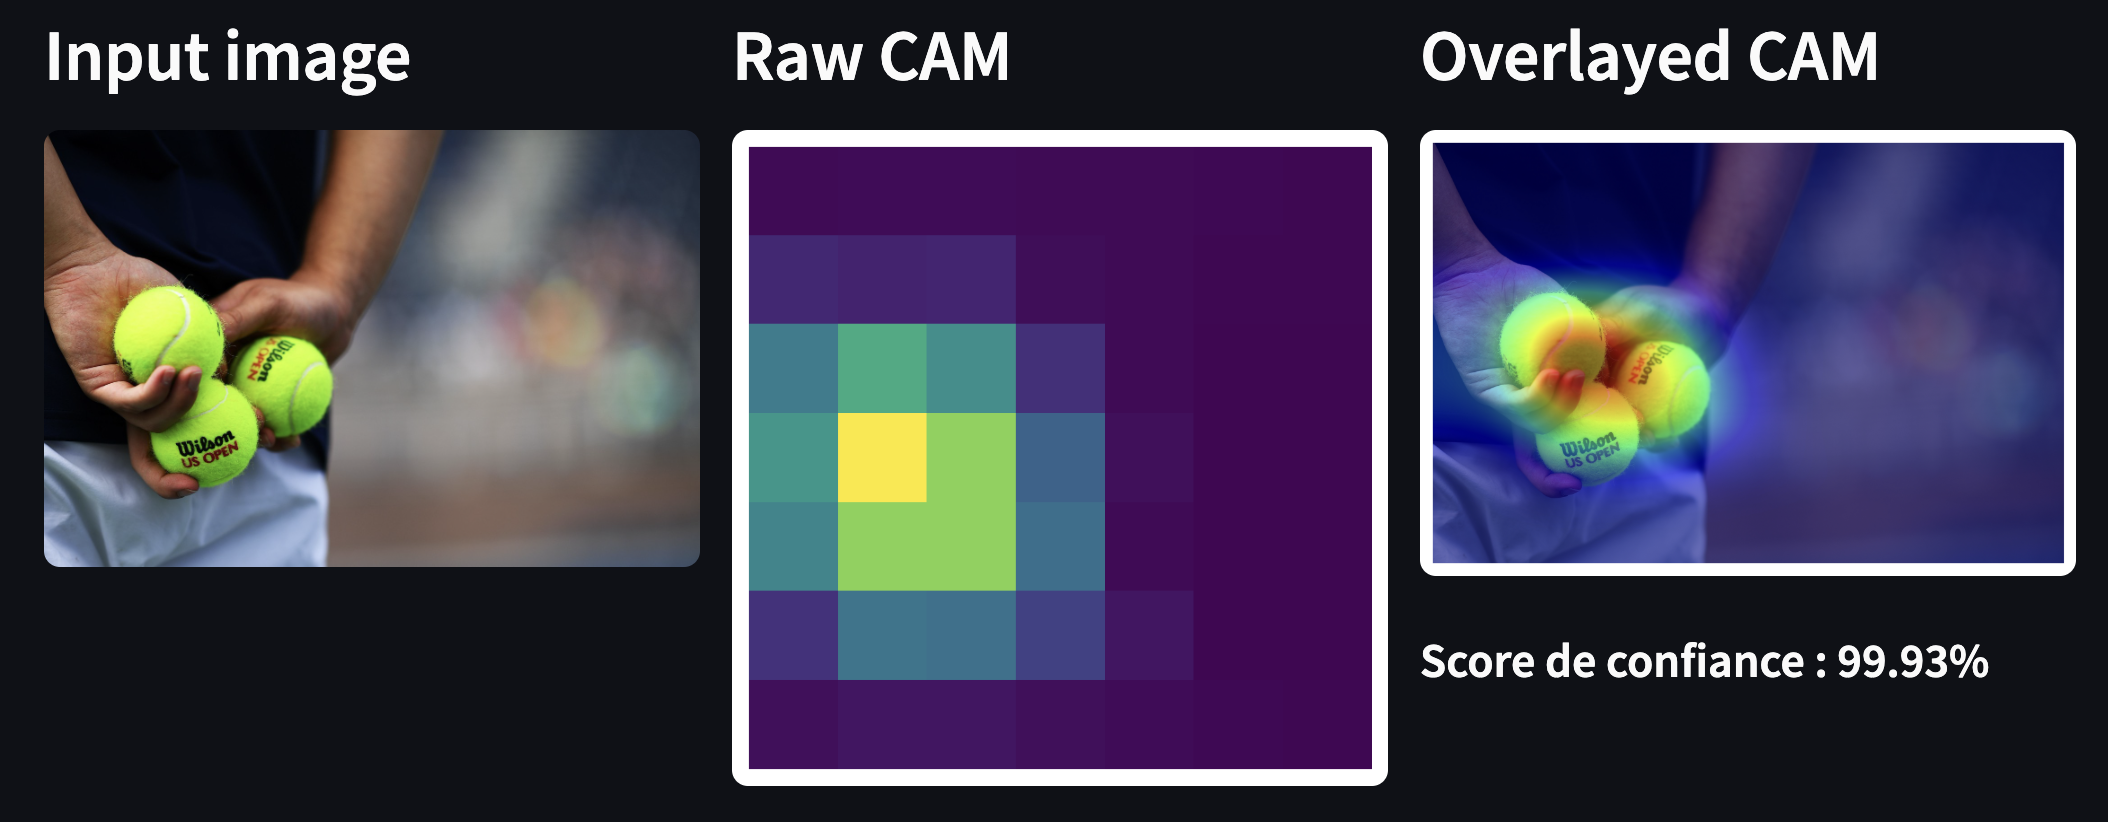
\includegraphics[width=0.9\linewidth]{CAM_tennis_balls.png}
    \caption{Résultat de l'activation pour plusieurs balles de tennis.}
\end{figure}
Pour l'image contenant plusieurs balles de tennis tenues dans une main, nous obtenons un score quasi-identique de \textbf{99.93\%}. Cela démontre la robustesse du modèle qui parvient à identifier correctement les balles de tennis même lorsqu'elles sont multiples et partiellement masquées. L'activation se concentre principalement sur les balles elles-mêmes plutôt que sur la main qui les tient, ce qui indique que le modèle a bien appris les caractéristiques distinctives des balles de tennis (texture, couleur, forme) et non le contexte environnant.

\begin{figure}[H]
    \centering
    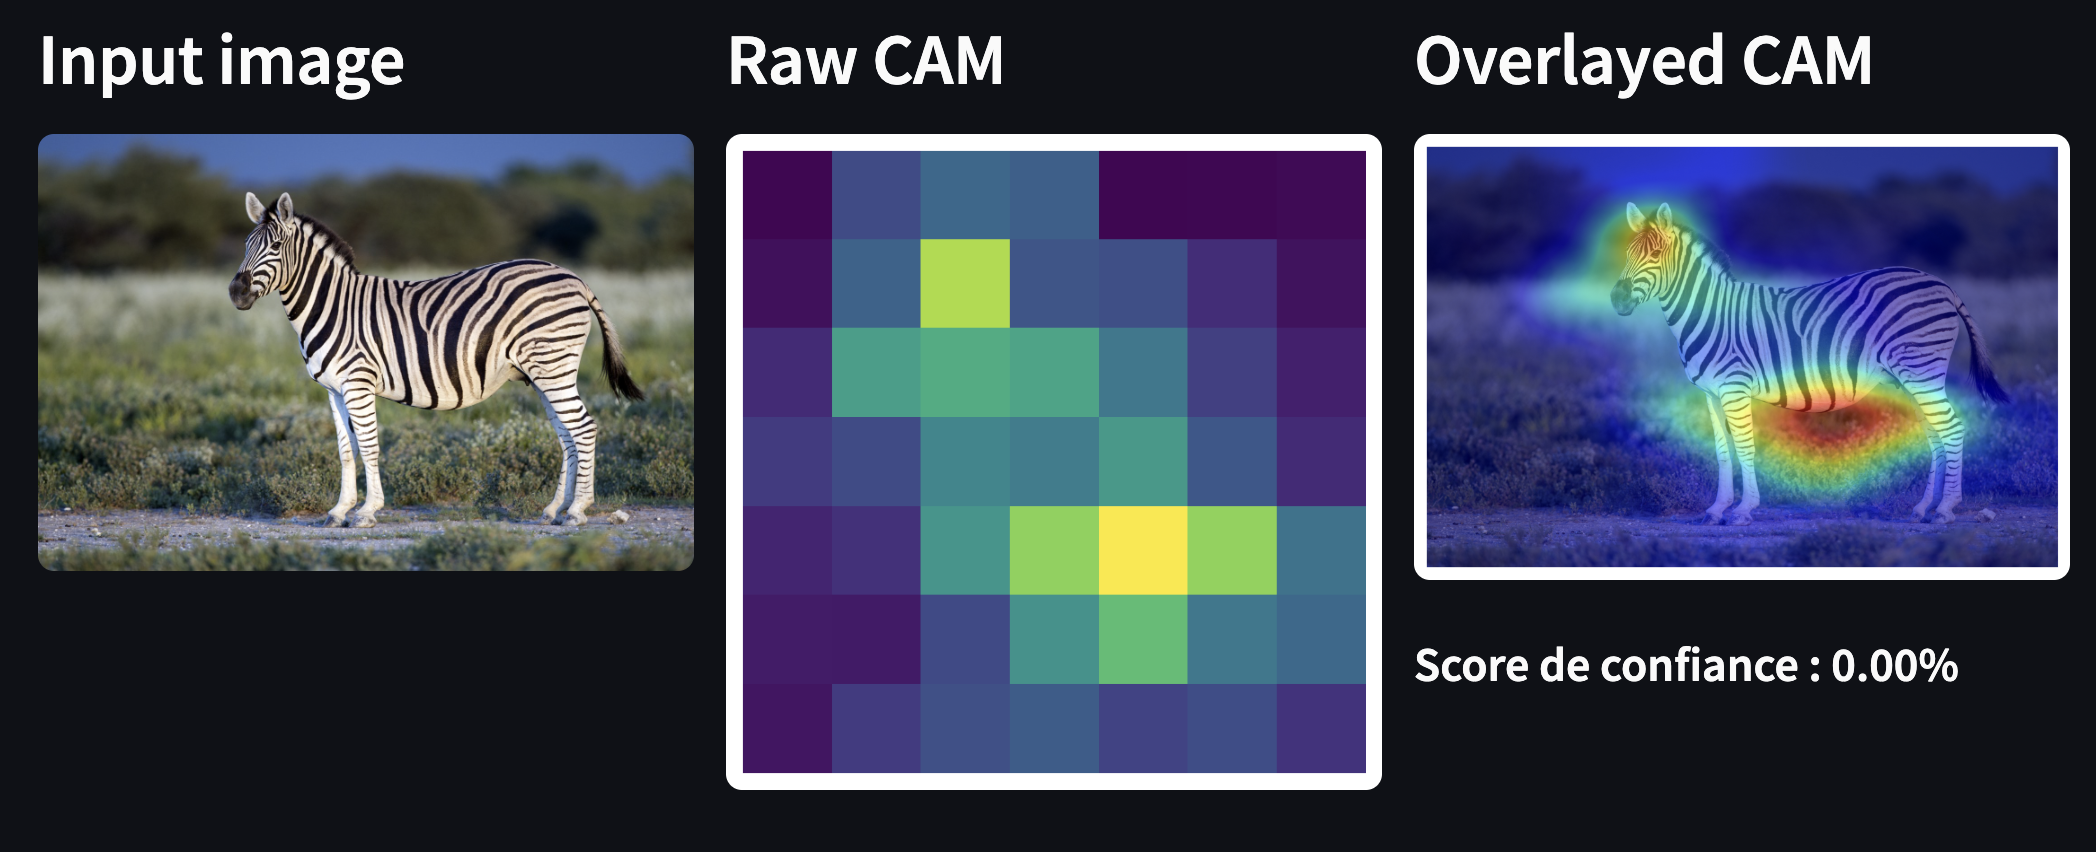
\includegraphics[width=0.9\linewidth]{CAM_zebra.png}
    \caption{Résultat de l'activation pour l'image d'un zèbre.}
\end{figure}
Enfin, pour l'image contenant un zèbre, le modèle retourne un score de confiance de \textbf{0.00\%}, indiquant correctement l'absence de balle de tennis. Il est intéressant de noter que malgré ce score nul, la carte thermique montre tout de même certaines activations, notamment autour de la tête du zèbre et sur certaines parties de son corps. Ces activations pourraient s'expliquer par la recherche par le modèle de formes arrondies ou de couleurs qui présentent des similitudes partielles avec les caractéristiques des balles de tennis.

\newpage
\subsubsection{Transformation de l'image}

Afin d'analyser plus profondément les performances et la fiabilité de notre modèle de détection d'objets, nous avons réalisé une série de tests en appliquant deux types distincts de transformations d'image (modification de luminosité et changement de perspective) sur notre image de référence contenant une unique balle de tennis. Cette approche nous permet d'évaluer la robustesse du modèle dans des conditions variables.\\\\
Pour chaque type de transformation, nous avons généré une séquence de 10 images présentant une intensité croissante de modification, permettant ainsi d'observer l'évolution progressive des performances du modèle face à ces altérations.

\begin{table}[H]
    \centering
    \begin{tabular}{|c|c|c|c|}
      \hline
      \textbf{Image} & \textbf{Score} & \textbf{Image} & \textbf{Score} \\
      \hline
      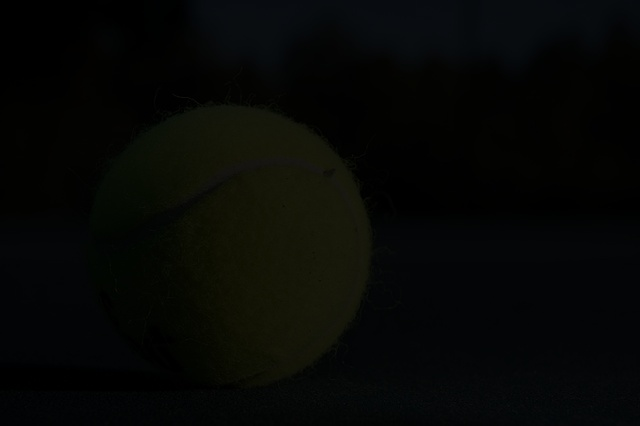
\includegraphics[width=0.25\textwidth]{images/brightness_1.jpg} & \Large 92.3 &
      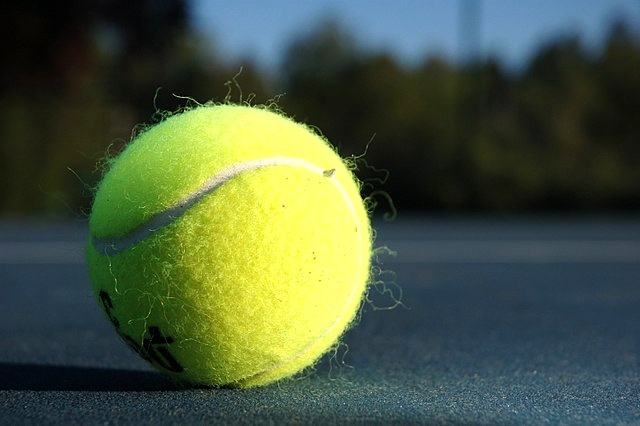
\includegraphics[width=0.25\textwidth]{images/brightness_2.jpg} & \Large 99.92 \\
      \hline
      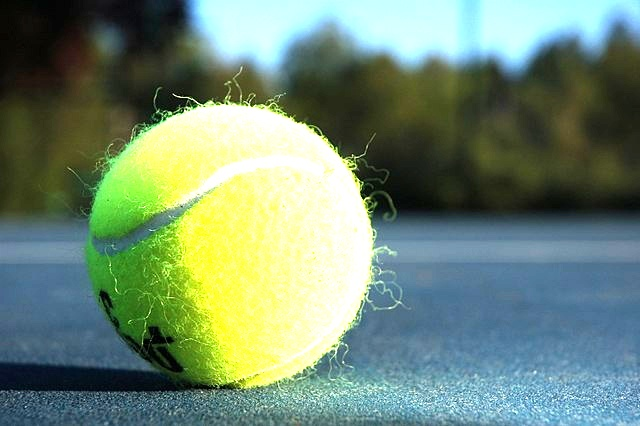
\includegraphics[width=0.25\textwidth]{images/brightness_3.jpg} & \Large 99.23 &
      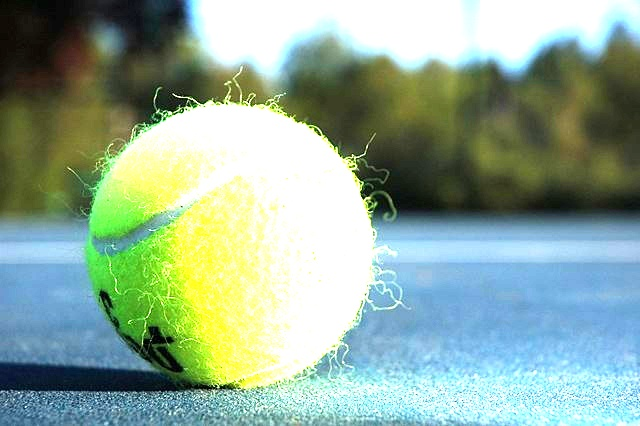
\includegraphics[width=0.25\textwidth]{images/brightness_4.jpg} & \Large 99.32 \\
      \hline
      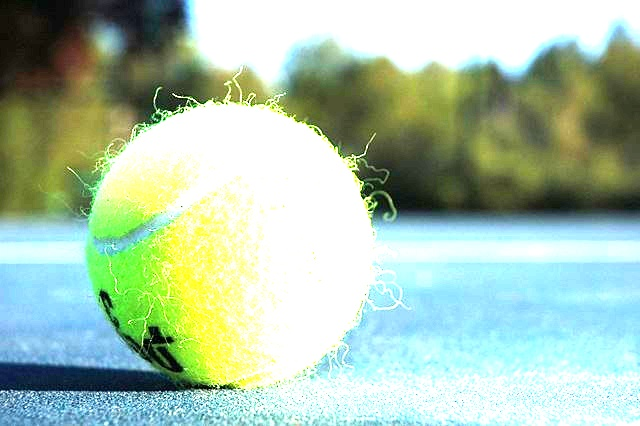
\includegraphics[width=0.25\textwidth]{images/brightness_5.jpg} & \Large 99.49 &
      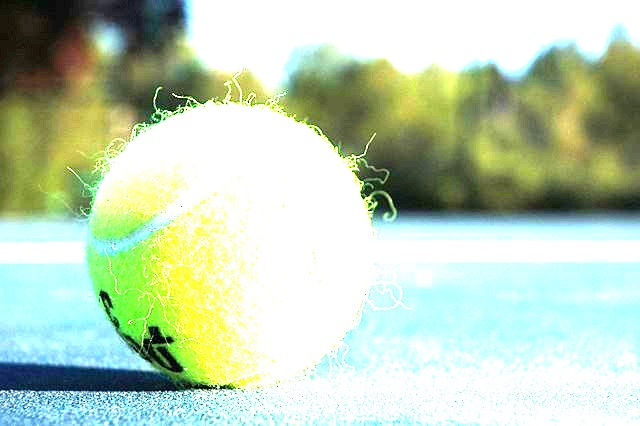
\includegraphics[width=0.25\textwidth]{images/brightness_6.jpg} & \Large 98.55 \\
      \hline
      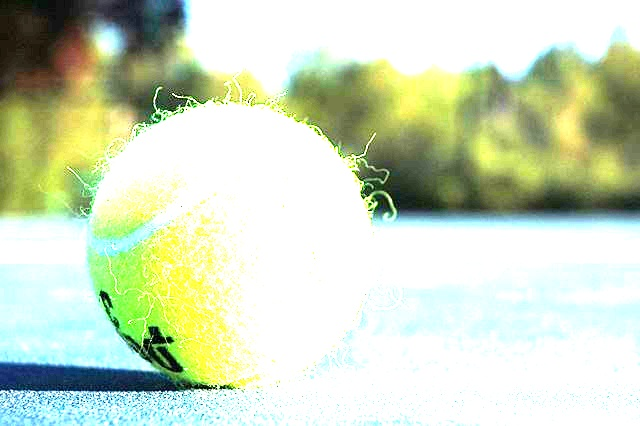
\includegraphics[width=0.25\textwidth]{images/brightness_7.jpg} & \Large 92.11 &
      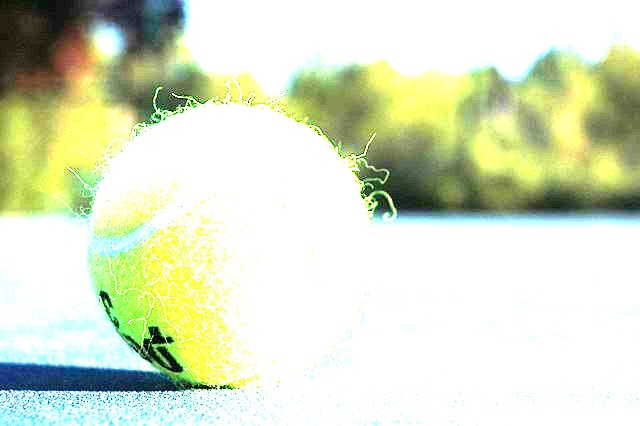
\includegraphics[width=0.25\textwidth]{images/brightness_8.jpg} & \Large 80.48 \\
      \hline
      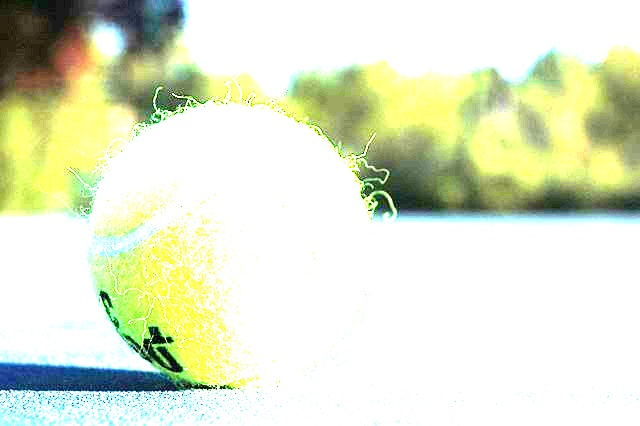
\includegraphics[width=0.25\textwidth]{images/brightness_9.jpg} & \Large 75.13 &
      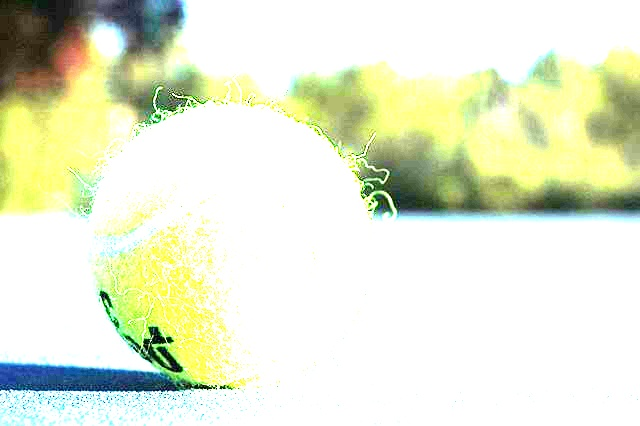
\includegraphics[width=0.25\textwidth]{images/brightness_10.jpg} & \Large 74.37 \\
      \hline
    \end{tabular}
    \caption{Comparaison des scores - luminosité}
    \label{tab:brightness_scores}
\end{table}

L'analyse des scores de confiance révèle plusieurs tendances significatives concernant la robustesse du modèle face aux variations de luminosité :

\begin{enumerate}
    \item Zone optimale de détection : Les scores les plus élevés ($>99\%$) sont obtenus pour les images avec une luminosité modérée (images 2 à 5), ce qui suggère une plage de fonctionnement optimal du modèle.
    \item Dégradation progressive : On observe une diminution notable des performances aux extrémités du spectre de luminosité :
    \begin{itemize}
        \item Pour les images très sombres (image 1), le score descend à 92.3\%
        \item Pour les images très lumineuses (images 7 à 10), on constate une dégradation encore plus marquée, avec des scores descendant jusqu'à 74.37\%
    \end{itemize}
    \item Seuil critique : La baisse significative des scores en dessous de 80\% pour les images fortement surexposées (images 9 et 10) indique un seuil critique au-delà duquel la fiabilité du modèle devient préoccupante.
\end{enumerate}

Cette tendance s'explique probablement par la perte de contraste et de détails caractéristiques de la balle de tennis dans les conditions extrêmes d'éclairage. Dans les images très lumineuses, la texture distinctive jaune-verte de la balle tend à se confondre avec l'arrière-plan en raison de la surexposition, tandis que dans les images très sombres, les contours et le contraste sont réduits.

\begin{table}[H]
    \centering
    \begin{tabular}{|c|c|c|c|}
      \hline
      \textbf{Image} & \textbf{Score} & \textbf{Image} & \textbf{Score} \\
      \hline
      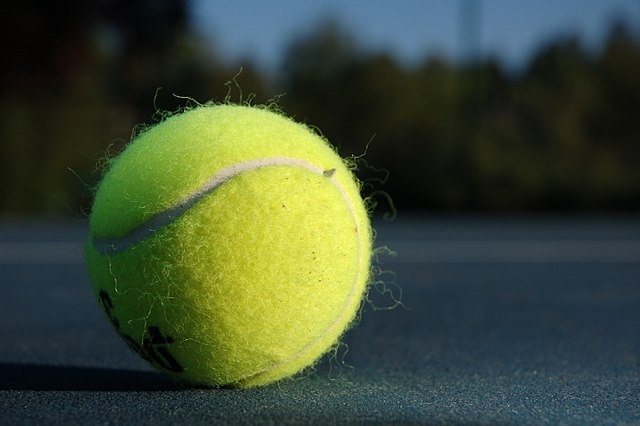
\includegraphics[width=0.25\textwidth]{images/perspective_1.jpg} & \Large 99.92 &
      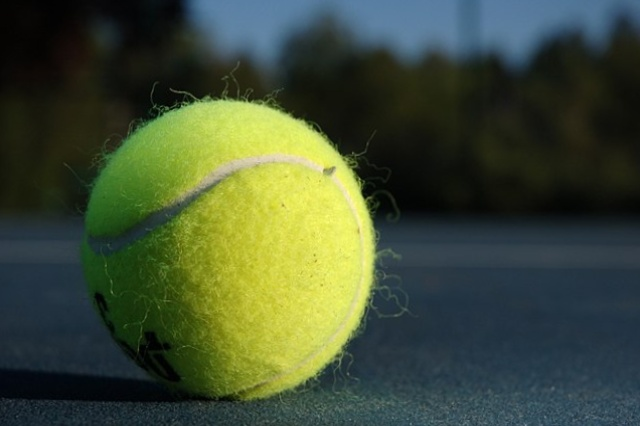
\includegraphics[width=0.25\textwidth]{images/perspective_2.jpg} & \Large 99.91 \\
      \hline
      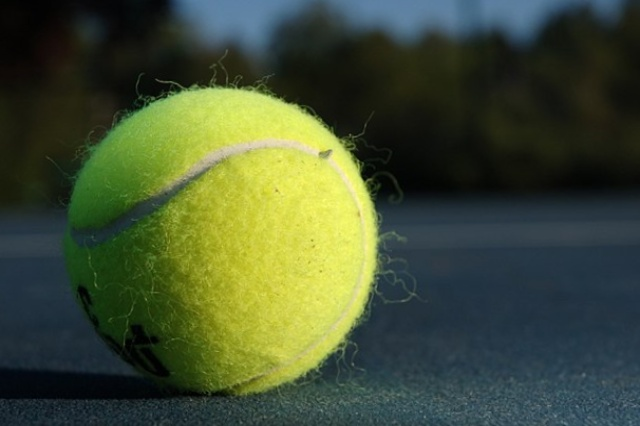
\includegraphics[width=0.25\textwidth]{images/perspective_3.jpg} & \Large 99.94 &
      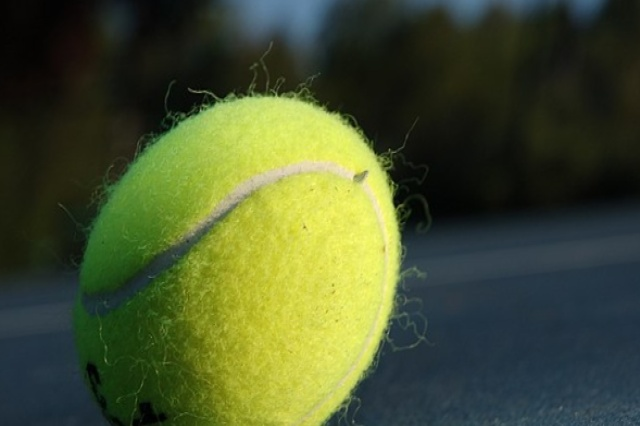
\includegraphics[width=0.25\textwidth]{images/perspective_4.jpg} & \Large 99.95 \\
      \hline
      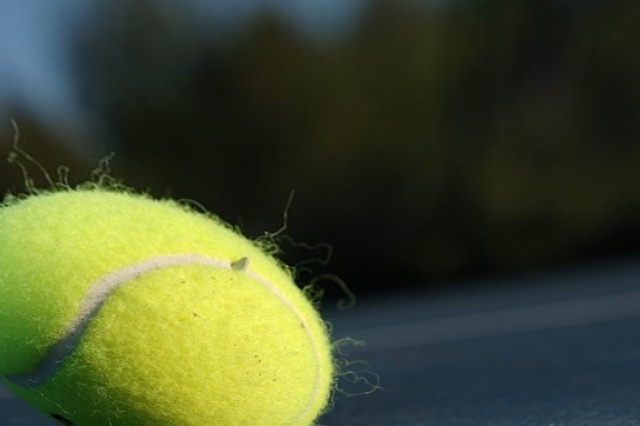
\includegraphics[width=0.25\textwidth]{images/perspective_5.jpg} & \Large 99.94 &
      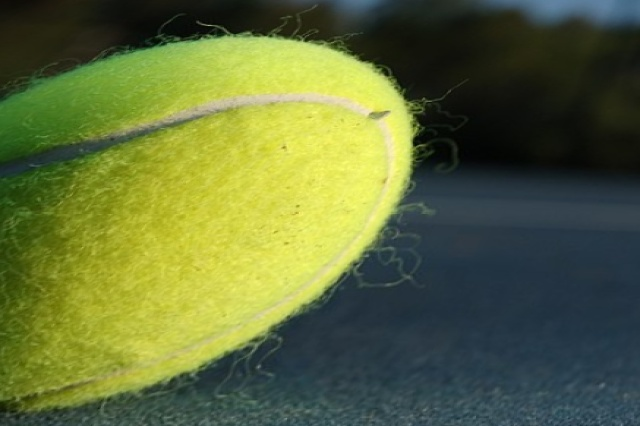
\includegraphics[width=0.25\textwidth]{images/perspective_6.jpg} & \Large 99.94 \\
      \hline
      
\includegraphics[width=0.25\textwidth]{images/perspective_7.jpg} & \Large 0.54 &
      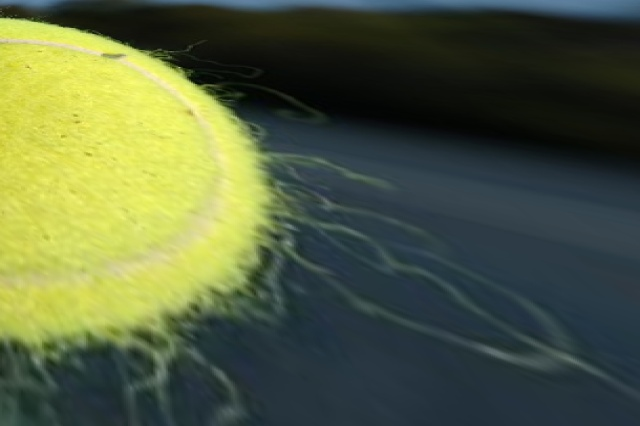
\includegraphics[width=0.25\textwidth]{images/perspective_8.jpg} & \Large 99.27 \\
      \hline
      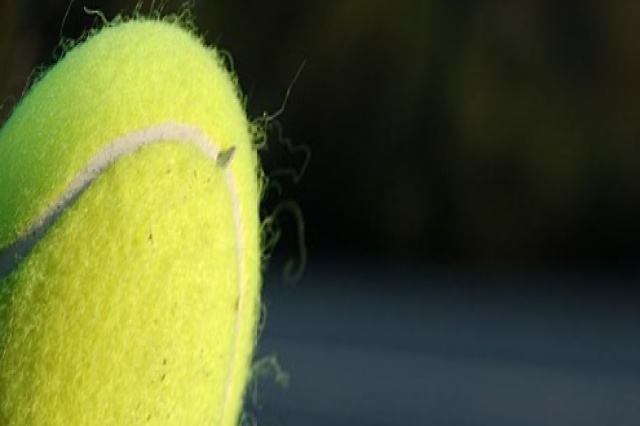
\includegraphics[width=0.25\textwidth]{images/perspective_9.jpg} & \Large 99.47 &
      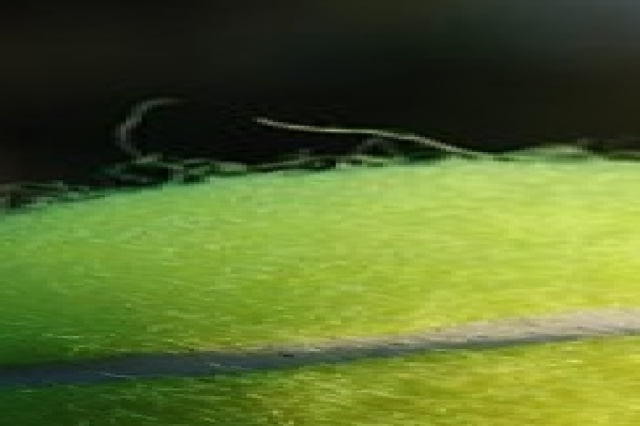
\includegraphics[width=0.25\textwidth]{images/perspective_10.jpg} & \Large 99.69 \\
      \hline
    \end{tabular}
    \caption{Comparaison des scores - perspective}
    \label{tab:perspective_scores}
\end{table}

L'analyse des scores de confiance pour les transformations de perspective révèle un comportement nettement différent de celui observé pour les variations de luminosité : 

\begin{enumerate}
    \item Haute robustesse générale : Le modèle démontre une remarquable stabilité face aux changements de perspective, avec des scores de confiance constamment supérieurs à 99\% pour 9 images sur 10. Cette performance suggère que les caractéristiques visuelles permettant l'identification de la balle de tennis sont invariantes à la plupart des transformations géométriques testées.
    \item Anomalie: L'image 7 présente une chute drastique du score de confiance (0.54\%), contrastant fortement avec les résultats des autres images de la série. Cela s'explique par le fait qu'on ne distingue plus la forme ronde de la balle de tennis dans cette image.
\end{enumerate}

\subsection{Conclusion}

D'après les expérimentations présentées, plusieurs observations importantes peuvent être faites concernant la sensibilité des réseaux de neurones convolutionnels (CNN) :

\begin{enumerate}
    \item Sensibilité différentielle aux types de transformations : Les résultats montrent clairement que le CNN testé réagit différemment selon le type de transformation appliquée. Il est considérablement plus sensible aux variations de luminosité qu'aux changements de perspective, ce qui suggère que les caractéristiques apprises par le réseau sont davantage liées aux propriétés de contraste et d'intensité lumineuse qu'aux aspects géométriques.
    \item Dégradation progressive vs défaillance abrupte : Pour les transformations de luminosité, on observe une dégradation graduelle des performances à mesure que l'on s'éloigne des conditions optimales, avec des scores passant progressivement de 99\% à 74\%. À l'inverse, pour les transformations de perspective, le modèle présente un comportement presque binaire : soit une reconnaissance excellente ($>99\%$), soit une défaillance complète (0.54\% pour l'image 7).
    \item Zones de fragilité spécifiques : L'analyse révèle des zones de fragilité particulières, notamment :
    \begin{itemize}
        \item Les conditions de forte surexposition (luminosité excessive)
        \item Certains angles de vue très spécifiques qui peuvent désorienter complètement le réseau
    \end{itemize}
\end{enumerate}

Nous pouvons conclure que les réseaux de neurones convolutionnels sont plus sensibles aux variations de lumière et de couleur qu'aux transformations géométriques telles que les rotations, les translations ou les changements d’échelle. Cette sensibilité s’explique par le fait que les CNN apprennent principalement à reconnaître des motifs et des textures spécifiques dans les images, plutôt que des formes abstraites indépendantes des conditions d’illumination. Ainsi, une modification de la luminosité ou de la teinte peut affecter significativement les activations des couches convolutionnelles, tandis qu’un changement d’orientation ou de position d’un objet dans l’image a généralement un impact plus faible, surtout si le modèle a été entraîné avec des données diversifiées. Cela met en évidence l'importance de techniques d'augmentation des données, comme la normalisation des couleurs ou l’application de transformations aléatoires, afin d’améliorer la robustesse des modèles de classification d’images aux variations de leur environnement.

\newpage
\begin{thebibliography}{9}
    \bibitem{kaggle} Jokekling, "PyTorch Study Audio", Kaggle, \url{https://www.kaggle.com/code/jokekling/pytorch-study-audio}
    \bibitem{audiomnist} Becker, S., Ackermann, M., Lapuschkin, S., Müller, K. R., \& Samek, W. (2018). "Interpreting and explaining deep neural networks for classification of audio signals." arXiv preprint arXiv:1807.03418.
    \bibitem{mel} Stevens, S. S., Volkmann, J., \& Newman, E. B. (1937). "A scale for the measurement of the psychological magnitude pitch." The Journal of the Acoustical Society of America, 8(3), 185-190.
    \bibitem{pytorch} Paszke, A., Gross, S., Massa, F., Lerer, A., Bradbury, J., Chanan, G., ... \& Chintala, S. (2019). "PyTorch: An imperative style, high-performance deep learning library." In Advances in Neural Information Processing Systems (pp. 8026-8037).
    \bibitem{youtube} Comprendre le DeepLearning et les Réseaux de neurones en 10 mins ! \url{https://www.youtube.com/watch?v=gPVVsw2OWdM}
    \bibitem{youtube} Coder un réseau de neurones convolutifs de classification d'image avec Python et Tensorflow. \url{https://www.youtube.com/watch?v=6FHtTyZxS5s}
\end{thebibliography}

\end{document}